%  LaTeX support: latex@mdpi.com 
%  For support, please attach all files needed for compiling as well as the log file, and specify your operating system, LaTeX version, and LaTeX editor.

%=================================================================
\documentclass[systems,article,submit,pdftex,moreauthors]{Definitions/mdpi} 
%\documentclass[preprints,article,submit,pdftex,moreauthors]{Definitions/mdpi} 
% For posting an early version of this manuscript as a preprint, you may use "preprints" as the journal. Changing "submit" to "accept" before posting will remove line numbers.


%=================================================================
% MDPI internal commands - do not modify
\firstpage{1} 
\makeatletter 
\setcounter{page}{\@firstpage} 
\makeatother
\pubvolume{1}
\issuenum{1}
\articlenumber{0}
\pubyear{2026}
\copyrightyear{2026}
%\externaleditor{Firstname Lastname} % More than 1 editor, please add `` and '' before the last editor name
\datereceived{ } 
\daterevised{ } % Comment out if no revised date
\dateaccepted{ } 
\datepublished{ } 
%\datecorrected{} % For corrected papers: "Corrected: XXX" date in the original paper.
%\dateretracted{} % For retracted papers: "Retracted: XXX" date in the original paper.
%\doinum{} % Used for some special journals, like molbank
%\pdfoutput=1 % Uncommented for upload to arXiv.org
%\CorrStatement{yes}  % For updates
%\longauthorlist{yes} % For many authors that exceed the left citation part
%\IsAssociation{yes} % For association journals



%=================================================================
% Add packages and commands here. The following packages are loaded in our class file: fontenc, inputenc, calc, indentfirst, fancyhdr, graphicx, epstopdf, lastpage, ifthen, float, amsmath, amssymb, lineno, setspace, enumitem, mathpazo, booktabs, titlesec, etoolbox, tabto, xcolor, colortbl, soul, multirow, microtype, tikz, totcount, changepage, attrib, upgreek, array, tabularx, pbox, ragged2e, tocloft, marginnote, marginfix, enotez, amsthm, natbib, hyperref, cleveref, scrextend, url, geometry, newfloat, caption, draftwatermark, seqsplit
% cleveref: load \crefname definitions after \begin{document}

%=================================================================
% Please use the following mathematics environments: Theorem, Lemma, Corollary, Proposition, Characterization, Property, Problem, Example, ExamplesandDefinitions, Hypothesis, Remark, Definition, Notation, Assumption
%% For proofs, please use the proof environment (the amsthm package is loaded by the MDPI class).

%=================================================================
% Full title of the paper (Capitalized)
\Title{Operational Data Foundation Framework for SME Smart Manufacturing: Field Implementation and Evidence}

% Author Orchid ID: enter ID or remove command
\newcommand{\orcidauthorA}{0009-0003-4190-193X}
\newcommand{\orcidauthorB}{0000-0001-6553-7448}

% Authors, for the paper (add full first names)
\Author{Yoonseok Kang $^{1}$\orcidA{} and Dongchul Park $^{2,}$*\orcidB{}}

%\longauthorlist{yes}

% MDPI internal command: Authors, for metadata in PDF
\AuthorNames{Yoonseok Kang and Dongchul Park}

%\longauthorlist{yes}

% Affiliations / Addresses (Add [1] after \address if there is only one affiliation.)
\address{%
$^{1}$ \quad Department of Convergence Security, Chung-Ang University, Seoul 06974, South Korea; kangcl1609@cau.ac.kr\\
$^{2}$ \quad Department of Industrial Security, Chung-Ang University, Seoul 06974, South Korea; dongchul@cau.ac.kr}

% Contact information of the corresponding author
\corres{Correspondence: dongchul@cau.ac.kr}
%; Tel.: (optional; include country code; if there are multiple corresponding authors, add author initials) +xx-xxxx-xxx-xxxx (F.L.)}




% Abstract (Do not insert blank lines, i.e. \\) 
\abstract{
Smart manufacturing increasingly depends on continuous and usable operational data, yet in constrained small and medium-sized enterprise (SME) factories, the practical bottleneck often lies not in downstream analytics or AI applications but in the absence of an operationally viable data foundation. This study addresses that problem by proposing an \emph{Operational Data Foundation Framework} for constrained SME manufacturing environments. The framework is derived from a lifecycle-based problem analysis and formalizes six core requirements: continuity, governance, diagnosability, operability, reprocessability, and evolvability. These requirements are further translated into design principles and operational invariants, thereby providing a structured basis for both design and assessment. To examine its field relevance, the framework was instantiated in a real SME deployment involving heterogeneous environmental sensors, a retrofitted legacy scale, LoRa-based field communication, edge-side persistence, cloud-side stream processing, and a governed canonical event model. The evaluation was conducted from the perspective of operational viability rather than benchmark performance alone. Requirement-based evidence showed that the implemented system preserved controlled semantics, supported segmented observability, maintained replayable historical records, and remained manageable under constrained deployment conditions. A representative field case further demonstrated the framework’s practical value: LoRa reception instability was diagnosed through segment-wise discrepancy analysis and improved from approximately 33\% to 95\% packet reception after targeted intervention. The study contributes a field-grounded design logic for operational data systems that can support monitoring, traceability, analytics, alerting, and future extensions in digitally constrained manufacturing settings.
}

% Keywords
\keyword{smart manufacturing; SME digitalization; industrial data infrastructure; data governance; edge–cloud architecture} 

%(List three to ten pertinent keywords specific to the article; yet reasonably common within the subject discipline.)

% The fields PACS, MSC, and JEL may be left empty or commented out if not applicable
%\PACS{J0101}
%\MSC{}
%\JEL{}






%%%%%%%%%%%%%%%%%%%%%%%%%%%%%%%%%%%%%%%%%%
\begin{document}

%%%%%%%%%%%%%%%%%%%%%%%%%%%%%%%%%%%%%%%%%%
%%%%%%%%%%%%%%%%%%%%%%%%%%%%%%%%%%%%%%%%%%
\section{Introduction}

Smart manufacturing is transforming manufacturing from a fixed and fragmented production environment into a connected operational system in which sensing, communication, computation, and decision making are tightly intertwined. Technologies such as the Internet of Things (IoT), cyber--physical systems (CPS), artificial intelligence and machine learning (AI/ML), real-time monitoring, predictive maintenance, and digital twins exemplify this shift. In this context, manufacturing systems can no longer be understood solely as physical production arrangements; they must also be understood as data-mediated operational systems.

Within this transition, data are no longer merely retrospective records. They have become a core operational resource that enables visibility, traceability, quality control, maintenance, optimization, and data-driven decision making. The practical advancement of smart manufacturing increasingly depends on whether operational data can be captured, interpreted, and reused in a stable and sustained manner across the shop floor. In this sense, smart manufacturing capability is closely tied to the continued availability of usable operational data.

At the same time, higher-level intelligent functions do not stand on their own. Predictive analytics, digital twins, and AI-driven optimization all presuppose an underlying operational layer that can continuously capture field data, preserve their meaning across system boundaries, and support downstream reuse. The central challenge, therefore, is not only what manufacturing systems can do more intelligently, but also which data conditions must first be maintained so that such intelligence becomes operationally viable.

The value of manufacturing data is not realized at the moment of generation alone. Rather, it emerges across an end-to-end flow that spans generation, acquisition, transmission, transformation, storage, and downstream use. For this reason, manufacturing data problems cannot be reduced to the performance of a single database, interface, or analytics component. They should instead be understood as operational systems problems distributed across the entire data lifecycle.

This challenge is intensified by the intrinsic heterogeneity of industrial data environments, where different devices, protocols, timestamps, machine states, manual records, and fragmented platforms coexist. Such conditions give rise to structural risks including missingness, duplication, delay, semantic inconsistency, timestamp ambiguity, and source-side variability. In manufacturing settings, these are not minor data imperfections. They directly affect traceability, weaken operational visibility, distort decision making, and ultimately reduce operational efficiency.

What is required, therefore, is not merely an ingestion infrastructure, but an operational layer capable of sustaining data continuity, governed semantics, durable persistence, observability, and downstream reusability. In this study, we refer to this layer as the \emph{operational data foundation}. The core issue is thus not simply whether data can be collected, but whether they can be maintained as an operationally usable and reusable resource. From this perspective, the operational data foundation should not be understood as a mere conduit for data movement. Rather, it provides the basis on which heterogeneous field data can be stabilized, governed, and made dependable for sustained operational and analytical use. As illustrated in Figure~\ref{fig:odf_position}, it occupies the intermediate layer between heterogeneous operational data sources and higher-level operational and analytical applications.


\begin{figure}[t]
    \centering
    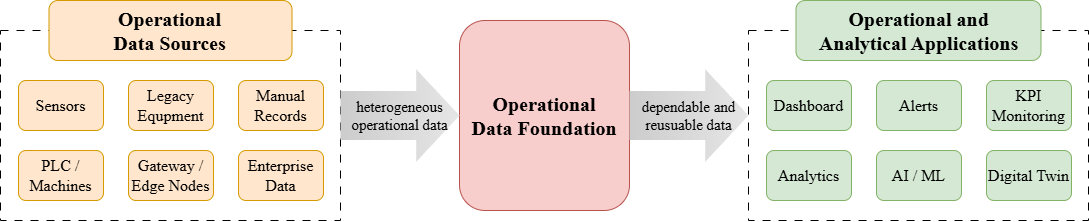
\includegraphics[width=\textwidth]{figures/1-2_Data_Froundation.png}
    \caption{Position of the operational data foundation in a digitalized manufacturing system.}
    \label{fig:odf_position}
\end{figure}

Although building dependable manufacturing data systems is challenging in general, its foundational requirements become especially visible in constrained small and medium-sized enterprise (SME) factories. These environments rarely offer the conditions often assumed in digitally mature smart-manufacturing settings, such as standardized interfaces, stable internal connectivity, dedicated technical support, and integrated data infrastructure. Instead, they more often combine legacy equipment, fragmented systems, mixed communication technologies, manual records, limited technical staffing, and strong cost sensitivity. For this reason, SME factories should not be regarded merely as smaller-scale plants, but as critical design settings in which the hidden assumptions of smart manufacturing data systems are exposed most clearly.

Under such conditions, the practical bottleneck of digitalization lies not simply in deploying more sensors, collecting more data, or adding downstream applications. Rather, it lies in whether operational data can be captured with continuity, stabilized with interpretable meaning, and sustained as a usable resource despite fragmentation, instability, and limited operational slack. In SME manufacturing, the central difficulty is therefore not merely data scarcity, but the fragility of the operational data lifecycle through which field data must become dependable for ongoing operational use.

This implies that the primary bottleneck of smart manufacturing in constrained SME factories lies not in downstream intelligence, but in establishing an operationally viable data foundation. Accordingly, this study addresses the following problem: \emph{how should an operational data foundation be designed, and what must it guarantee, in order to make smart manufacturing practically viable in constrained SME factories?}

Existing research has addressed manufacturing data systems from several complementary directions. Smart manufacturing studies have primarily focused on higher-level applications and intelligent capabilities, including real-time monitoring, predictive maintenance, digital twins, and adaptive production support. In parallel, research on industrial data infrastructures has examined pipelines, integration architectures, edge--cloud coordination, semantic consistency, governance, and data quality. Related lifecycle-oriented work has emphasized continuity, traceability, reusable linkage, and the preservation of context across stages, while studies on SME digitalization have clarified the realities of constrained deployment, including legacy equipment, fragmented systems, limited staffing, and strong cost sensitivity.

However, these contributions remain only partially integrated from the perspective of operational viability under constrained deployment conditions. Prior work has often addressed applications, architectural components, lifecycle properties, or SME deployment constraints as related but separate concerns, rather than formalizing what a manufacturing data foundation must guarantee in order to remain operationally usable in practice. As a result, there is still limited systems-level articulation of how these interrelated concerns can be brought together into a coherent design basis for constrained SME manufacturing environments.

To address this gap, this study focuses on the foundational layer that smart manufacturing applications presuppose and formalizes it in terms of operational requirements, design logic, and verification basis. More specifically, this study develops an \emph{Operational Data Foundation Framework} for constrained SME factories and examines it through field-grounded implementation and evidence.

Based on this motivation, the study is guided by the following research questions:

\begin{itemize}
    \item \textbf{RQ1.} What operational risks emerge when smart manufacturing data pipelines are deployed under constrained SME factory conditions?
    \item \textbf{RQ2.} What core requirements must an operational data foundation satisfy in such conditions, and how can they be formalized into design principles and operational invariants?
    \item \textbf{RQ3.} How can the proposed framework be instantiated in a real SME manufacturing setting, and how can its practical value be examined through field evidence?
\end{itemize}

To answer these questions, this study first organizes a general lifecycle model of smart manufacturing data pipelines as an analytical reference. It then maps constrained SME factory conditions onto that lifecycle in order to identify the key operational risks that hinder practical deployment. In response to these risks, the study formalizes the Operational Data Foundation Framework in terms of core requirements, design principles, and operational invariants. Finally, it instantiates the framework in a real SME manufacturing setting and examines its practical value through requirement-based evidence and representative field observations.

The primary contributions of this research are as follows:
\begin{enumerate}
    \item Redefining the actual bottleneck of smart manufacturing in constrained SME factories not as a downstream application problem, but as an operational data foundation problem.
    \item Deriving the core operational risks that emerge when a general manufacturing data lifecycle is subjected to constrained SME factory conditions.
    \item Formalizing the Operational Data Foundation Framework (ODFF), structured around core requirements, design principles, and operational invariants.
    \item Validating the framework's field-grounded operational relevance through real-world implementation in an SME manufacturing environment.
\end{enumerate}

The remainder of this paper is organized as follows. Section~2 reviews the related literature. Section~3 analyzes the general data pipeline lifecycle, SME-specific constraints, and the resulting operational risks. Section~4 presents the proposed Operational Data Foundation Framework. Section~5 describes the field implementation in an SME manufacturing setting. Section~6 evaluates the framework using requirement-based evidence and field observations. Finally, Section~7 concludes the paper.


%%%%%%%%%%%%%%%%%%%%%%%%%%%%%%%%%%%%%%%%%%
%%%%%%%%%%%%%%%%%%%%%%%%%%%%%%%%%%%%%%%%%%
\section{Related Work}

%%%%%%%%%%%%%%%%%%%%%%%%%%%%%%%%%%%%%%%%%%
\subsection{Smart Manufacturing Applications}

Smart manufacturing research has developed mainly around higher-level applications and intelligent capabilities, including industrial IoT, cyber--physical systems, digital twins, real-time monitoring, predictive maintenance, and AI/ML-enabled decision making \cite{rozhok2026advanced, bueno2020smart, cinar2020digital, atalay2022digital}. Across these streams, the dominant goal has been to make manufacturing systems more connected, adaptive, and data-driven through improved visibility, prediction, and control \cite{rozhok2026advanced, bueno2020smart, song2025smart}.

Despite their diversity, these applications share a common prerequisite: continuous or near-real-time operational data from the shop floor \cite{nguyen2025aidriven, tao2017digital, ding2019digital}. Studies on digital twins and real-time manufacturing intelligence repeatedly show that higher-level functions depend on accurate, timely, and interpretable data aligned with physical system states \cite{nguyen2025aidriven, ojstersek2023optimizing, qamsane2019digital}. Yet this literature is generally more explicit about what smart manufacturing applications can optimize, predict, or automate than about what kind of data basis must first be sustained for those functions to remain operationally viable in practice \cite{rozhok2026advanced, ciano2021digital, nguyen2025aidriven}.

%%%%%%%%%%%%%%%%%%%%%%%%%%%%%%%%%%%%%%%%%%
\subsection{Industrial Data Infrastructures}

A substantial body of research has examined the industrial data basis through manufacturing data pipelines, integration architectures, industrial data management systems, and edge--cloud infrastructures \cite{ismail2019manufacturing, raptis2019data, saqlain2019framework}. This literature makes clear that manufacturing data handling is not a single storage problem, but a multi-layer systems problem spanning acquisition, communication, processing, storage, and downstream delivery across heterogeneous sources \cite{ismail2019manufacturing, odonovan2015industrial}.

Within this stream, two themes are especially prominent. First, many studies address heterogeneous integration and interoperability across legacy equipment, devices, protocols, platforms, and enterprise systems \cite{zeid2019interoperability, pereira2021towards, modoni2017enhancing}. Second, related work has emphasized semantics, context, and governance, arguing that industrial data must remain interpretable, trustworthy, and reusable rather than merely transferable \cite{hildebrandt2020ontology, morris2020foundations, westermann2022accessing}. These contributions have significantly advanced the understanding of how industrial data infrastructures can be connected, organized, and managed. However, they remain more focused on components, architectures, and enabling techniques than on explicitly formalizing what such infrastructures must guarantee as an operational foundation under deployment constraints \cite{ismail2019manufacturing, raptis2019data, morris2020foundations}.

%%%%%%%%%%%%%%%%%%%%%%%%%%%%%%%%%%%%%%%%%%
\subsection{Lifecycle Connectivity}

This view has been developed most clearly through the concept of the digital thread. Recent reviews and implementation studies define the digital thread as a means of linking lifecycle information across heterogeneous artifacts and stages, thereby enabling traceability, cross-stage visibility, and reuse beyond isolated system silos \cite{abdelaty2024conceptualizing, zhang2024digitalthread, bianchini2024digitalthread, hedberg2020graphs}. Related work on contextualization, standards-based linkage, and knowledge-graph integration similarly shows that lifecycle usefulness depends not only on storing data, but on preserving associativity, context, and interpretability for later reuse \cite{kwon2020enriching, schmidt2018flow, monnier2022methodology}. However, this literature has focused mainly on linkage and traceability, leaving relatively less explicit discussion of how such continuity and reuse can be sustained operationally under constrained deployment conditions.

The concept of the digital thread has become the clearest expression of this perspective. Recent reviews and implementation studies define the digital thread as a means of linking information across heterogeneous lifecycle artifacts and stages so that traceability, cross-stage visibility, and lifecycle-wide reuse become possible beyond fragmented system silos \cite{abdelaty2024conceptualizing, zhang2024digitalthread, bianchini2024digitalthread, hedberg2020graphs}. Related studies on contextualization, standards-based linkage, and knowledge-graph integration likewise show that lifecycle usefulness depends not merely on storing records, but on preserving associativity, context, and interpretability for later reuse \cite{kwon2020enriching, schmidt2018flow, monnier2022methodology}. At the same time, this literature has concentrated mainly on linkage and traceability, leaving relatively less explicit discussion of how such continuity and reuse can be sustained operationally under constrained deployment conditions.

%%%%%%%%%%%%%%%%%%%%%%%%%%%%%%%%%%%%%%%%%%
\subsection{SME Deployment}

The SME literature makes those deployment constraints explicit. Studies on smart manufacturing adoption in SMEs consistently show that these environments differ substantially from idealized smart factory assumptions: legacy equipment, fragmented systems, uneven interfaces, limited digital infrastructure, restricted investment capacity, and uneven technical expertise are common \cite{mittal2018maturity, mittal2020adoption, ghobakhloo2019adoption, krishnan2024challenges}. In this sense, SMEs should not be viewed simply as smaller large factories, but as constrained deployment settings in which the assumptions of digitally mature architectures are most directly challenged.

This constraint is both technical and operational. Brownfield dependence often forces SMEs to rely on retrofitting, add-on sensing, gateway-based integration, and low-cost connectivity rather than wholesale replacement \cite{alqoud2022legacy, etz2020retrofit, tran2022retrofitting, park2019opcua}. At the same time, recurrent barriers include limited staffing, weak digital skills, uncertain return on investment, high implementation cost, and maintainability burden \cite{huang2025barriers, narwane2022examining, kumar2025digitalization, hulla2021towards}. Accordingly, SME-oriented studies increasingly advocate phased, modular, and capability-building adoption paths \cite{chavez2020capability, krishnan2024challenges, banerjee2024lowcost}. Taken together, these studies show that the unresolved problem is not how to deploy smart manufacturing application, infrastructure component, or lifecycle linkage mechanism, but how to sustain a data foundation that remains operationally viable under constrained real-world conditions.


%%%%%%%%%%%%%%%%%%%%%%%%%%%%%%%%%%%%%%%%%%
%%%%%%%%%%%%%%%%%%%%%%%%%%%%%%%%%%%%%%%%%%
\section{Problem Analysis}

This section analyzes the data basis of smart manufacturing as an operational pipeline and examines how constrained SME factory conditions impose structural fragility across that pipeline. Rather than merely describing deployment difficulty, it identifies how lifecycle-wide constraints converge into a small set of recurring operational risks. In this way, the section defines the problem structure of operational data foundations under constrained deployment conditions.

%%%%%%%%%%%%%%%%%%%%%%%%%%%%%%%%%%%%%%%%%%
\subsection{General Data Pipeline Lifecycle}

\begin{figure}
    \centering
    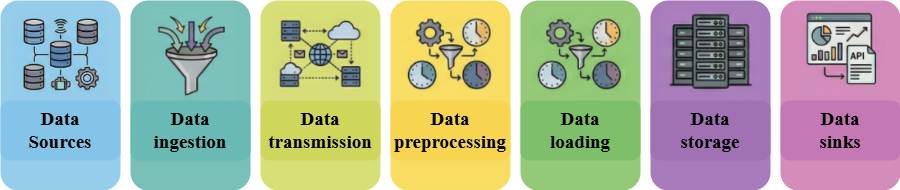
\includegraphics[width=1\linewidth]{figures/3-1_Data_Lifecycle.png}
    \caption{General data pipeline lifecycle in smart manufacturing.}
    \label{fig:data_lifecycle}
\end{figure}


A common analytical reference is required before constrained SME conditions and their resulting risks can be examined in a structured way. In smart manufacturing, data do not become operationally useful at the moment of generation alone. Their practical value emerges only through a broader path in which field observations are accepted into a pipeline, transferred across infrastructure layers, transformed into usable forms, preserved, and connected to downstream operational use. For this reason, this study adopts a \emph{general data pipeline lifecycle} as an analytical frame for problem interpretation rather than as a normative system architecture.

The lifecycle used in this study is shown in Figure~\ref{fig:data_lifecycle}. It is adapted from generic data pipeline literature that treats data systems as multi-stage processing structures with recurring issues around ingestion, integration, cleaning, transformation, loading, and pipeline-wide quality control \cite{foidl2024pipeline}. In the smart manufacturing context, this general view is organized as follows:

\begin{itemize}
    \item \textbf{Data sources:} the points at which operational data originate, including sensors, equipment states, manual records, and external systems.
    \item \textbf{Data ingestion:} the intake of source data into the pipeline.
    \item \textbf{Data transmission:} the movement of acquired data across gateway, edge, server, or cloud boundaries toward the next processing point.
    \item \textbf{Data preprocessing:} the cleaning, decoding, normalization, mapping, and transformation required to make raw inputs usable downstream.
    \item \textbf{Data loading:} the controlled insertion of processed records into the target operational layer or storage boundary.
    \item \textbf{Data storage:} the durable preservation of records for later access, recovery, reinterpretation, and reuse.
    \item \textbf{Data sinks:} the downstream endpoints that consume stored data, including dashboards, alerts, reporting, analytics, and decision support.
\end{itemize}

This lifecycle is analytically useful because it makes visible the full path through which manufacturing data become operationally usable. At the same time, it is not a design answer on its own. It describes how data move, but not what must be preserved so that the lifecycle remains operationally viable under constrained conditions. It is therefore used in this study as an analytical reference for the constraint and risk analysis that follows.


%%%%%%%%%%%%%%%%%%%%%%%%%%%%%%%%%%%%%%%%%%
\subsection{SME Constraints}

\begin{figure}
    \centering
    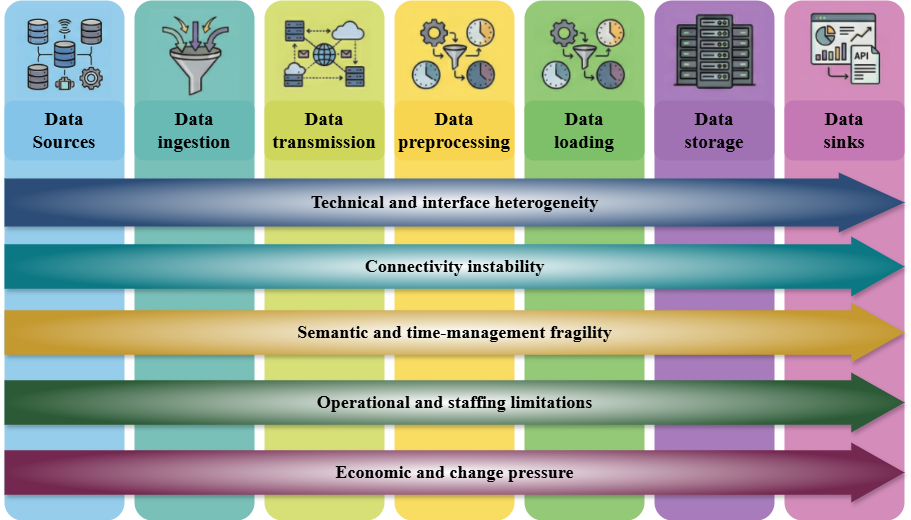
\includegraphics[width=1\linewidth]{figures/3-2_Data_Lifecycle.png}
    \caption{SME constraints across the general data pipeline lifecycle.}
    \label{fig:3-2_data_lifecycle}
\end{figure}


Constrained SME factories should not be treated simply as smaller versions of digitally mature plants. Prior research shows that their starting conditions are structurally different: legacy equipment, fragmented systems, uneven interfaces, restricted digital infrastructure, limited internal expertise, and strong investment sensitivity are common, whereas standardized connectivity and unified data access are often absent \cite{mittal2018maturity, mittal2020adoption, ghobakhloo2019adoption, krishnan2024challenges, rauch2019requirements}. SME constraints are therefore better understood not as isolated implementation difficulties, but as recurring design conditions acting across the general data pipeline lifecycle. Figure~\ref{fig:3-2_data_lifecycle} highlights this point by showing how the major constraint types propagate across source capture, transfer, transformation, storage, and downstream use rather than remaining confined to a single stage.

Heterogeneity begins at the source side. In SME factories, brownfield machinery, retrofit-based extension, add-on sensing, and gateway-mediated access are common, so inconsistency is already present at the level of data sources and ingestion rather than appearing only later in integration \cite{alqoud2022legacy, etz2020retrofit, tran2022retrofitting, park2019opcua}. The challenge is not merely collecting values, but incorporating diverse formats, units, reporting intervals, and source identities into a coherent operational structure. Source-side variability is thus not a peripheral inconvenience, but the starting condition from which later coordination and interpretation problems arise.

Transmission is often fragile in constrained SME deployments. In constrained SME deployments, field data may depend on low-cost wireless communication, battery-powered sensing, and gateway- or edge-dependent relay paths rather than on stable plant-wide infrastructure \cite{gao2019connectivity, noor2023wireless, hawkridge2019tying}. The ingestion--transmission path therefore becomes a distinct surface of instability. What matters operationally is not simply whether a value was observed once, but whether the record can remain sufficiently continuous and recoverable despite interruption, delay, and relay dependence.

Operational meaning must remain stable across the pipeline. Manufacturing data are operationally usable only when source identity, metric semantics, unit interpretation, and time semantics stay controlled across preprocessing, loading, and storage. Yet constrained environments frequently rely on heterogeneous preprocessing logic, ad hoc mappings, incomplete context, and weak contract discipline, making semantic drift and traceability loss structurally likely \cite{pereira2021towards, nagorny2020rami, hildebrandt2020ontology, westermann2022accessing, morris2020foundations}. Once such instability becomes embedded in stored records, downstream analytics and dashboards may continue to function while resting on an increasingly fragile semantic basis.

These technical difficulties are intensified by operational reality. SME studies repeatedly report limited staffing, uneven digital skills, manual troubleshooting, high maintenance burden, and weak strategic capacity \cite{huang2025barriers, kumar2025digitalization, hulla2021towards, nasirinejad2024maintenance}. At the same time, SME digitalization rarely proceeds as a one-shot transformation; it unfolds through phased rollout, retrofit-based extension, KPI revision, and incremental onboarding of new sources and processes \cite{chavez2020capability, doyle2019steps, mcfarlane2022digitalisation, banerjee2024lowcost}. As a result, the practical challenge is not only whether a system can be built, but whether it can remain diagnosable, manageable, and adaptable as requirements change.

Taken together, these observations show that the core problem in constrained SME factories is not simply that deployment is difficult. Rather, the assumptions of the general data pipeline lifecycle are systematically destabilized across the lifecycle itself: records may lose continuity, meanings may drift, failures may become hard to localize, operational burden may grow, historical data may lose replay value, and later extension may require disproportionate rework. The next subsection translates these recurring forms of fragility into the language of operational risk.



%%%%%%%%%%%%%%%%%%%%%%%%%%%%%%%%%%%%%%%%%%
\subsection{Operational Risks}

The SME constraints discussed above do not remain as isolated deployment difficulties. When mapped onto the general data pipeline lifecycle, they appear as recurring operational risks that determine whether manufacturing data can remain usable in practice. The issue is therefore not only how data move through the pipeline, but what must be preserved so that the resulting record remains dependable under constrained real-world conditions.

\begin{itemize}[leftmargin=1.5em]
    \item[\textbf{RSK1.}] \textbf{Continuity risk.} Operational records may become interrupted, fragmented, or partially lost as data move from source capture to storage. In constrained manufacturing settings, the essential requirement is not one-time collection success, but the preservation of a gap-minimized and recoverable record despite source instability, transmission disruption, or delayed recovery.

    \item[\textbf{RSK2.}] \textbf{Governance risk.} Data may remain available while losing stable meaning. This occurs when source identity, metric semantics, timestamp interpretation, or transformation logic are not kept consistent across collection, preprocessing, loading, and storage. Under such conditions, downstream analysis may continue to operate, but on data whose meaning is no longer reliably governed.

    \item[\textbf{RSK3.}] \textbf{Diagnosability risk.} When failure occurs, it may be difficult to determine where in the lifecycle the problem emerged and what kind of failure it is. Weak monitoring, poor stage separation, and limited observability turn degradation into a black-box symptom, making it difficult to distinguish transmission loss, semantic corruption, storage inconsistency, or downstream mismatch in a structurally interpretable way.

    \item[\textbf{RSK4.}] \textbf{Operability risk.} A system may function technically while becoming too costly or complex to sustain in everyday practice. Tight coupling, heavy maintenance burden, unclear ownership, and non-modular structures raise the effort required to manage, modify, and repair the system, making long-term operation difficult under constrained SME staffing and budget conditions.

    \item[\textbf{RSK5.}] \textbf{Reprocessability risk.} Historical data may cease to be usable when rules, KPIs, schemas, or interpretation logic change. If raw preservation is weak, preprocessing is effectively irreversible, or lineage is incomplete, past records cannot be reliably replayed, recomputed, or reinterpreted. In that case, the data foundation loses one of its most important operational values: the ability to support correction and renewed interpretation over time.

    \item[\textbf{RSK6.}] \textbf{Evolvability risk.} New sensors, processes, lines, factories, or downstream requirements may become difficult to incorporate without disproportionate redesign cost or structural disruption. Since SME digitalization usually proceeds through incremental onboarding rather than one-shot integration, a data foundation that cannot absorb change without breaking governance and operational control cannot serve as a durable basis for growth.
\end{itemize}

Taken together, these risks show that a smart manufacturing data pipeline in constrained SME factories cannot be treated as a simple ingestion flow. The problem is not a collection of isolated device, network, or software issues, but a structural fragility of the lifecycle through which operational data become usable. What is required, therefore, is a foundation that can explicitly preserve continuity, governance, diagnosability, operability, reprocessability, and evolvability under constrained deployment conditions. The next section presents the \emph{Operational Data Foundation Framework} as a structured response to these risks.


%%%%%%%%%%%%%%%%%%%%%%%%%%%%%%%%%%%%%%%%%%
%%%%%%%%%%%%%%%%%%%%%%%%%%%%%%%%%%%%%%%%%%
\section{Operational Data Foundation Framework}

%%%%%%%%%%%%%%%%%%%%%%%%%%%%%%%%%%%%%%%%%%
\subsection{Framework Overview}

\begin{figure}
    \centering
    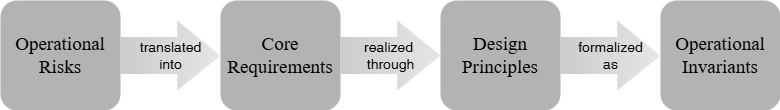
\includegraphics[width=1\linewidth]{figures/4-1_Framework.png}
    \caption{Operational Data Foundation Framework.}
    \label{fig:4-1_framework}
\end{figure}

Section~3 showed that, in constrained SME factory environments, smart manufacturing data pipelines are exposed to recurring risks of continuity loss, semantic instability, weak diagnosability, operational burden, limited reprocessability, and poor evolvability. These risks indicate that the data layer cannot be treated merely as a transmission path or collection mechanism. What is needed instead is an explicit framework that defines what an operational data foundation must guarantee in order to remain viable under constrained deployment conditions.

To address this need, this study proposes the \emph{Operational Data Foundation Framework}. As shown in Figure~\ref{fig:4-1_framework}, the framework is organized as a risk-to-design logic: \emph{operational risks} are translated into \emph{core requirements}; these requirements are realized through \emph{design principles}; and their realized state is assessed through \emph{operational invariants}. In this way, the framework converts the problem structure identified in Section~3 into an explicit and assessable basis for the design and evaluation of an operational data foundation.
%%%%%%%%%%%%%%%%%%%%%%%%%%%%%%%%%%%%%%%%%%
\subsection{Core Requirements}

The framework begins by defining the \emph{core requirements} of an operational data foundation. These requirements are not desirable properties in a general sense, but the minimum lifecycle-wide guarantees needed for operational viability under constrained SME factory conditions. They provide the basis for the design principles and operational invariants developed in the following subsections.

Six core requirements are defined.

\begin{itemize}
    \item[\textbf{R1.}] \textbf{Continuity.} Data continuity should be preserved as far as practicable despite field disruption and connectivity instability. The essential requirement is not momentary acquisition success, but the minimization of gaps and the preservation of recoverable continuity so that the operational record remains usable even when intermediate segments are unstable.

    \item[\textbf{R2.}] \textbf{Governance.} Source identity, metric semantics, and time semantics should remain stable across collection, normalization, and storage. Data are not operationally usable merely because they exist; they must retain controlled meaning and interpretable context throughout the pipeline.

    \item[\textbf{R3.}] \textbf{Diagnosability.} Failures should be observable as segment-level discrepancies rather than only as end-to-end symptoms. The requirement is not simply that problems become visible after damage appears downstream, but that the lifecycle location and mode of failure can be identified in a structurally interpretable way.

    \item[\textbf{R4.}] \textbf{Operability.} The system should remain maintainable and manageable under constrained staffing and budget conditions. An operational data foundation must therefore be sustainable in day-to-day practice without imposing structurally excessive maintenance burden or operational complexity.

    \item[\textbf{R5.}] \textbf{Reprocessability.} Historical data should remain reprocessable for rule changes, KPI revisions, correction, and recovery. Manufacturing data should not be treated as one-time consumables, but as records that can be read again, recalculated, and reinterpreted when operational needs evolve.

    \item[\textbf{R6.}] \textbf{Evolvability.} The foundation should accommodate new sources, processes, sites, and applications without breaking the existing structure. Since SME digitalization typically proceeds through incremental onboarding rather than one-time integration, the data foundation must remain structurally open to change and extension.
\end{itemize}

%%%%%%%%%%%%%%%%%%%%%%%%%%%%%%%%%%%%%%%%%%
\subsection{Design Principles}

The core requirements defined above specify what the operational data foundation must guarantee, but not how those guarantees should be realized in design. This subsection therefore presents the key \emph{design principles} that translate those requirements into a workable design logic for constrained SME factory conditions. Rather than prescribing specific technologies or implementation choices, these principles define the structural directions needed to sustain the required operational guarantees.

\begin{itemize}
    \item[\textbf{P1.}] \textbf{Continuity responsibility should be placed close to the source.} If continuity depends primarily on downstream transmission or cloud reachability, it becomes fragile under field disruption and connectivity instability. For this reason, the first responsibility for preserving continuity should be located as close to the source as possible through source-near capture, upstream buffering or persistence, and recovery-oriented ingestion logic.

    \item[\textbf{P2.}] \textbf{Raw events should be preserved before abstraction.} If only transformed outputs are retained, later replay, reinterpretation, and recovery become structurally limited. The preservation of raw events before irreversible abstraction is therefore a fundamental design principle, since rule changes, KPI revision, and correction all depend on access to preserved pre-abstraction records.

    \item[\textbf{P3.}] \textbf{Semantics should be contract-defined.} If source identity, metric naming, timestamp semantics, unit definition, and transformation logic are left to ad hoc implementation, semantic inconsistency accumulates across the pipeline. The design must therefore define semantics explicitly through controlled contracts, schema discipline, version-aware rules, and clear identity and time conventions.

    \item[\textbf{P4.}] \textbf{Observability should follow pipeline segments.} Diagnosability cannot be secured through black-box end-to-end monitoring alone, because operationally meaningful failures must be localizable to specific lifecycle segments. Observability should therefore be structured along the pipeline itself through segment-wise checkpoints, stage-level indicators, and explicit discrepancy visibility.

    \item[\textbf{P5.}] \textbf{Responsibilities should be separated by function.} If acquisition, normalization, storage, and downstream use are tightly coupled, both maintenance burden and change cost rise rapidly. Functional responsibilities should therefore be separated so that components remain structurally independent, interfaces remain replaceable, and modifications in one part do not unnecessarily destabilize the whole.

    \item[\textbf{P6.}] \textbf{Operations should remain lightweight, modular, and open.} In constrained SME environments, heavy operational structures, costly maintenance models, and vendor dependence undermine long-term viability. The design should therefore remain lightweight in deployment, modular in composition, manageable in maintenance scope, and open to replacement and extension. Where appropriate, open and widely supported components, including open-source tools, can help reduce lock-in and maintenance burden.
    
    \item[\textbf{P7.}] \textbf{Change should be treated as a first-class assumption.} Changes in KPIs, schemas, rules, source onboarding, and deployment scope are not exceptional events but normal operating conditions in SME digitalization. The foundation should therefore be designed from the outset to tolerate and organize change through version-aware structures, replay support, incremental onboarding discipline, and change-tolerant interfaces.
\end{itemize}

%%%%%%%%%%%%%%%%%%%%%%%%%%%%%%%%%%%%%%%%%%
\subsection{Operational Invariants}

The core requirements and design principles defined above specify what the operational data foundation must guarantee and how those guarantees should be realized. This subsection completes the framework by defining the \emph{operational invariants}: the persistent conditions that should hold if the foundation is functioning as intended.

\begin{itemize}
    \item[\textbf{I1.}] \textbf{Durable Capture Invariant.} An accepted event should obtain durable persistence before downstream failure can erase it. Continuity should therefore be judged from the point of first durable capture rather than from downstream availability alone.

    \item[\textbf{I2.}] \textbf{Traceability Invariant.} Every canonical or stored record should remain traceable to its source identity and operational context. Downstream data should not become detached from the source, metadata, and governing semantics that give it meaning.

    \item[\textbf{I3.}] \textbf{Deterministic Normalization Invariant.} The same raw event under the same contract and version conditions should always produce the same canonical output. Normalization should function as a repeatable and controlled semantic transformation rather than as ad hoc interpretation.

    \item[\textbf{I4.}] \textbf{Segment-Localizable Failure Invariant.} A failure should become visible as at least one discrepancy within a recognizable lifecycle segment. It should be possible to attribute the problem to a specific segment such as source, transmission, preprocessing, loading, storage, or sink rather than observing it only as a downstream symptom.

    \item[\textbf{I5.}] \textbf{Replayability Invariant.} Preserved raw data should remain reprocessable for rule changes, KPI revision, correction, and recovery. Historical data should therefore remain usable for later reinterpretation and recomputation rather than serving only as passive archive material.

    \item[\textbf{I6.}] \textbf{Modular Replacement Invariant.} Replacing a specific component should not break the semantic chain of the overall foundation. Changes in storage, parsing, transport, or downstream components should not destroy source identity, metric meaning, or replay context across the system.

    \item[\textbf{I7.}] \textbf{Onboarding Consistency Invariant.} A new source should be incorporable into the existing structure without breaking the prevailing governance discipline. Incremental onboarding should proceed through the same contract, schema, naming, and validation discipline rather than through an accumulation of ad hoc exceptions.
\end{itemize}

These invariants define the persistent conditions by which the framework can be assessed in practice. If requirements declare the guarantees to be achieved and principles define the design logic needed to achieve them, invariants provide the basis for evaluating whether those guarantees remain structurally preserved.

%%%%%%%%%%%%%%%%%%%%%%%%%%%%%%%%%%%%%%%%%%
\subsection{Framework Synthesis}

This subsection synthesizes the framework by reconnecting it to the problem space analyzed in Section~3. Section~3 showed how constrained SME factory conditions destabilize the general data pipeline lifecycle and generate recurring risks of continuity, governance, diagnosability, operability, reprocessability, and evolvability. Sections~4.2--4.4 translated those risks into core requirements, design principles, and operational invariants. The purpose here is to clarify how these layers are systematically linked to the original problem structure.

Table~\ref{tab:constraint_design_logic} provides this first synthesis. It shows that constrained SME conditions are not merely a list of deployment difficulties, but recurring operational design problems that can be translated in a structured way. Each major constraint category gives rise to one or more operational risks; each risk is then expressed as a core requirement, translated into one or more design principles, and made assessable through corresponding invariants. The table thus shows how the framework is grounded in recurring structural problems in constrained SME manufacturing.


\begin{table}[H]
\caption{From SME constraints to operational design logic.\label{tab:constraint_design_logic}}
\begin{adjustwidth}{-\extralength}{0cm}
\begin{tabularx}{\fulllength}{
>{\raggedright\arraybackslash}X
>{\raggedright\arraybackslash}X
>{\raggedright\arraybackslash}X
>{\raggedright\arraybackslash}X
>{\raggedright\arraybackslash}X}
\toprule
\textbf{SME Constraint} & \textbf{Operational Risk} & \textbf{Requirement} & \textbf{Design Principle} & \textbf{Invariant} \\
\midrule

Heterogeneous devices and fragmented interfaces
& RSK2 (Governance risk)
& R2 (Governance)
& P3 (Semantics must be contract-defined)
& I2 (Traceability), I3 (Deterministic normalization) \\

Add-on sources and partial visibility
& RSK2, RSK6 (Evolvability risk)
& R2, R6 (Evolvability)
& P3, P7 (Change as a first-class assumption)
& I2, I7 (Onboarding consistency) \\

Unstable connectivity and constrained sensing
& RSK1 (Continuity risk)
& R1 (Continuity)
& P1 (Continuity responsibility must be placed close to the source)
& I1 (Durable capture) \\

Weak cross-segment observability
& RSK3 (Diagnosability risk)
& R3 (Diagnosability)
& P4 (Observability must follow pipeline segments)
& I4 (Segment-localizable failure) \\

Limited staff and high maintenance burden
& RSK4 (Operability risk)
& R4 (Operability)
& P6 (Operations must remain lightweight, modular, and open)
& I6 (Modular replacement) \\

Weak raw-data preservation
& RSK5 (Reprocessability risk)
& R5 (Reprocessability)
& P2 (Raw events must be preserved before abstraction)
& I5 (Replayability) \\

Tight functional coupling across the pipeline
& RSK3, RSK4, RSK6
& R3, R4, R6
& P5 (Responsibilities must be separated by function)
& I4, I6 \\

Frequent KPI, rule, schema, and source changes
& RSK5, RSK6
& R5, R6
& P7
& I5, I7 \\

Budget sensitivity and lock-in concerns
& RSK4, RSK6
& R4, R6
& P6
& I6, I7 \\

\bottomrule
\end{tabularx}
\end{adjustwidth}
\end{table}




One particularly important translation highlighted in Table~\ref{tab:constraint_design_logic} is the movement from semantic and interface heterogeneity to governance logic. In constrained SME factories, heterogeneous devices, mixed protocols, fragmented interfaces, add-on sensing, and manual records do not merely create diverse formats; they destabilize source identity, metric meaning, unit interpretation, and timestamp semantics. The issue is therefore not simply one of integration, but one of governance. For this reason, the framework connects this problem to \emph{R2 Governance}, \emph{P3 contract-defined semantics}, and the assessable conditions of \emph{I2 Traceability} and \emph{I3 Deterministic Normalization}. This translation makes clear that manufacturing data become operationally reliable only when meaning and origin remain stably governed.

A second important translation concerns the movement from change pressure to reprocessability and evolvability logic. SME digitalization rarely proceeds as a one-time integration event; instead, KPI definitions evolve, schemas change, new sensors and lines are added, and operational rules are revised over time. When such change is not treated as a normal operating condition, transformed-only persistence and weak lineage make past data difficult to reinterpret and new sources difficult to onboard without exception-heavy modification. The framework therefore connects this problem to \emph{R5 Reprocessability} and \emph{R6 Evolvability}, supported by \emph{P7 change as a first-class assumption} and assessed through \emph{I5 Replayability} and \emph{I7 Onboarding Consistency}. This shows that the framework is designed not only for present-time correctness, but also for preserving operational coherence under future change.

Table~\ref{tab:lifecycle_foundation_logic} provides a second synthesis by showing how the framework adds operational meaning to the general data pipeline lifecycle. Under constrained SME conditions, each lifecycle stage must contribute not only to data movement and processing, but also to the guarantees defined by the operational data foundation. The table makes this added meaning explicit by connecting each stage to the relevant risks, requirements, design principles, and invariants. In this way, the general lifecycle is retained as an analytical reference, while its role is sharpened for constrained manufacturing conditions.

One especially revealing example is the reinterpretation of the transmission stage. In generic pipeline discussions, transmission is often treated as a routine internal link between ingestion and later processing. In constrained SME factory conditions, however, the path from field devices to gateways, edge systems, servers, and cloud systems is often exposed to intermittent connectivity, limited bandwidth, battery constraints, delayed recovery, and relay dependence. Transmission therefore becomes a distinct operational segment in which continuity and diagnosability are directly tested. For this reason, Table~\ref{tab:lifecycle_foundation_logic} assigns the transmission stage the added meanings of recoverable transfer and segment-aware discrepancy visibility, linking it to \emph{R1 Continuity}, \emph{R3 Diagnosability}, \emph{P1 source-near continuity}, \emph{P4 segment-based observability}, \emph{I1 Durable Capture}, and \emph{I4 Segment-Localizable Failure}.

Taken together, Table~\ref{tab:constraint_design_logic} translates constrained SME conditions into operational design logic, while Table~\ref{tab:lifecycle_foundation_logic} shows how that logic refines the interpretation of the general data pipeline lifecycle under real manufacturing constraints. The result is a single analytical structure that connects problem space, framework logic, and lifecycle interpretation. This synthesis also provides the basis for reading the field implementation in Section~5 and the evidence assessment in Section~6.






\begin{table}[H]
\caption{Mapping the general data pipeline lifecycle to the operational foundation logic.\label{tab:lifecycle_foundation_logic}}
\begin{adjustwidth}{-\extralength}{0cm}
\begin{tabularx}{\fulllength}{
>{\raggedright\arraybackslash}X
>{\raggedright\arraybackslash}X
>{\raggedright\arraybackslash}X
>{\raggedright\arraybackslash}X
>{\raggedright\arraybackslash}X
>{\raggedright\arraybackslash}X}
\toprule
\textbf{General Lifecycle Stage} & \textbf{Added Operational Meaning} & \textbf{Related Risks} & \textbf{Requirements} & \textbf{Principles} & \textbf{Invariants} \\
\midrule

Data sources
& Stable source identity
& RSK2, RSK6
& R2, R6
& P3, P7
& I2, I7 \\

Data ingestion
& Source-near continuity and intake control
& RSK1, RSK2
& R1, R2
& P1, P3
& I1, I2 \\

Data transmission
& Recoverable transfer and visible discrepancies
& RSK1, RSK3
& R1, R3
& P1, P4
& I1, I4 \\

Data preprocessing
& Contract-defined and deterministic transformation
& RSK2, RSK6
& R2, R6
& P3, P7
& I2, I3, I7 \\

Data loading
& Controlled persistence with replay context
& RSK5, RSK6
& R5, R6
& P2, P7
& I5, I7 \\

Data storage
& Replay-ready and replaceable persistence
& RSK4, RSK5
& R4, R5
& P2, P6
& I5, I6 \\

Data sinks
& Governed downstream reuse
& RSK2, RSK5
& R2, R5
& P3, P7
& I2, I5 \\

Monitoring and management across the lifecycle
& Lifecycle-wide observability and maintainability
& RSK3, RSK4
& R3, R4
& P4, P6
& I4, I6 \\

\bottomrule
\end{tabularx}
\end{adjustwidth}
\end{table}



%%%%%%%%%%%%%%%%%%%%%%%%%%%%%%%%%%%%%%%%%%
%%%%%%%%%%%%%%%%%%%%%%%%%%%%%%%%%%%%%%%%%%
\section{Field Implementation}

This section describes how the proposed framework was instantiated in a real SME manufacturing setting. The implementation is presented not as a generic IoT deployment, but as a field realization of an operational data foundation under constrained conditions. The focus is therefore placed on how heterogeneous sources were incorporated, how continuity was secured close to the source, how semantics were stabilized through the processing and storage path, and how the resulting data layer was connected to operational visibility and intervention.

%%%%%%%%%%%%%%%%%%%%%%%%%%%%%%%%%%%%%%%%%%
\subsection{Plant Context and Sensing Objectives}

\begin{figure}
    \centering
    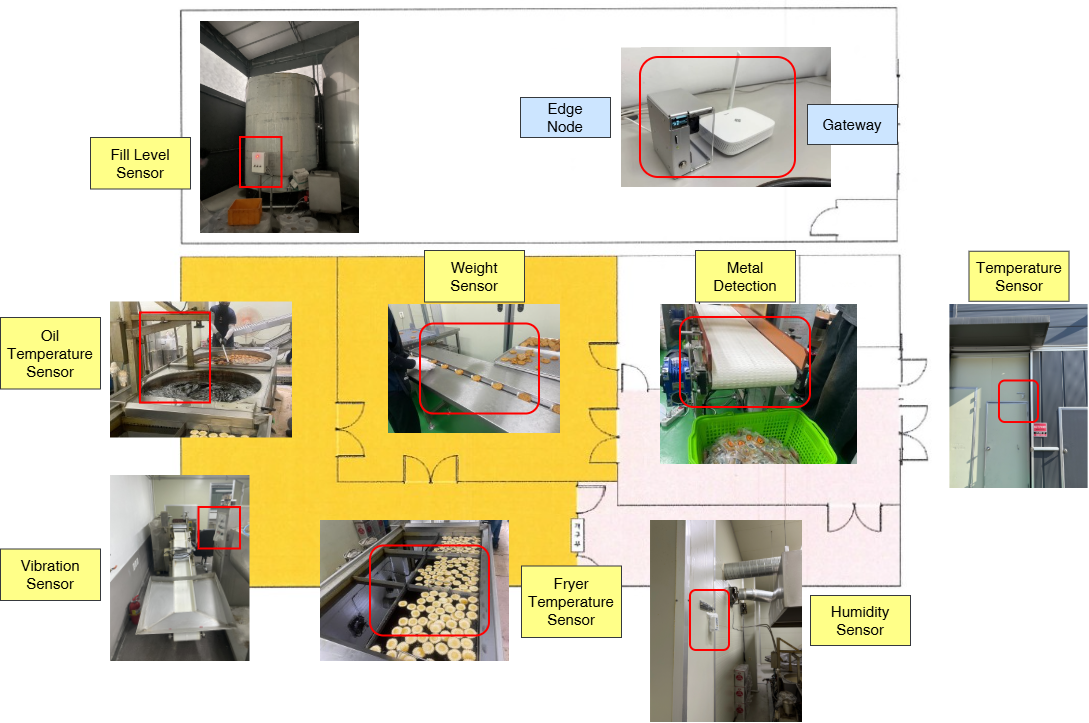
\includegraphics[width=1\linewidth]{figures/5-1_Factory.png}
    \caption{Factory layout with representative sensing and edge deployment.}
    \label{fig:5-1_factory}
\end{figure}

The empirical setting of this study was the Idang Food yakgwa plant, one of several OEM factories managed by ONGOING, an F\&B company operating across multiple production sites. The deployment was therefore designed not as an isolated factory pilot, but as the first field implementation of a broader architecture in which operational data from multiple factories could be collected locally and managed through a shared cloud-side structure. In this sense, Idang Food was selected not only as a practical implementation site, but also as a representative case through which this study examines how an operational data foundation can be established under constrained SME manufacturing conditions.

The plant's production flow included raw-material receiving, weighing, mixing, forming, frying, coating, cooling, inner packaging, detection, outer packaging, and storage. Yet the main challenge of the site did not lie simply in the number of stages. Operationally relevant states were distributed across different rooms, devices, and tasks, while production and quality management depended heavily on manual records and worker judgement. Process conditions were not accumulated as connected records, weighing-related checks remained strongly operator-dependent, and environmental histories across process and storage zones were difficult to preserve and compare over time. As a result, when abnormal conditions or quality issues emerged, the plant did not lack observations in an absolute sense; rather, it lacked continuous and reusable operational records that could support traceability and later interpretation.

This made the site suitable for the present study. Idang Food reflected several conditions that commonly characterize constrained SME factories: heterogeneous and partly non-networked sources, fragmented process visibility, limited internal connectivity, and restricted operational slack for day-to-day technical management. Under such conditions, an operational data foundation could not be assumed to arise simply from downstream software or cloud connectivity. It first had to be built from the field upward by making process states recordable, collectable, and sustainable as data under actual production constraints.

The field deployment should be understood in this light. The study did not begin from an already prepared digital source environment, but from the practical requirement to establish one inside the factory through on-site sensing and edge-side installation. Figure~\ref{fig:5-1_factory} presents this deployment context by showing the production environment together with representative sensing and edge elements installed in the field. The significance of the case, however, lies less in the installation itself than in what that installation enabled: a concrete demonstration of how a constrained SME factory can begin to acquire the operational basis required for continuity, traceability, and later cloud-side integration.

Accordingly, the role of Idang Food in this study was twofold. At the factory level, it provided a realistic constrained environment in which fragmented sources, manual practices, and brownfield conditions had to be handled in practice. At the system level, it served as the first implementation site of an architecture intended to support factory-to-cloud data flow and centralized multi-factory management. For this reason, the next subsection begins with field data acquisition and the edge architecture, because the first requirement of the operational data foundation was to explain how field data were physically captured and operationally secured at the factory before they were forwarded into the broader cloud-side system.

%%%%%%%%%%%%%%%%%%%%%%%%%%%%%%%%%%%%%%%%%%
\subsection{Field Data Acquisition and Edge Stack}

\begin{figure}
    \centering
    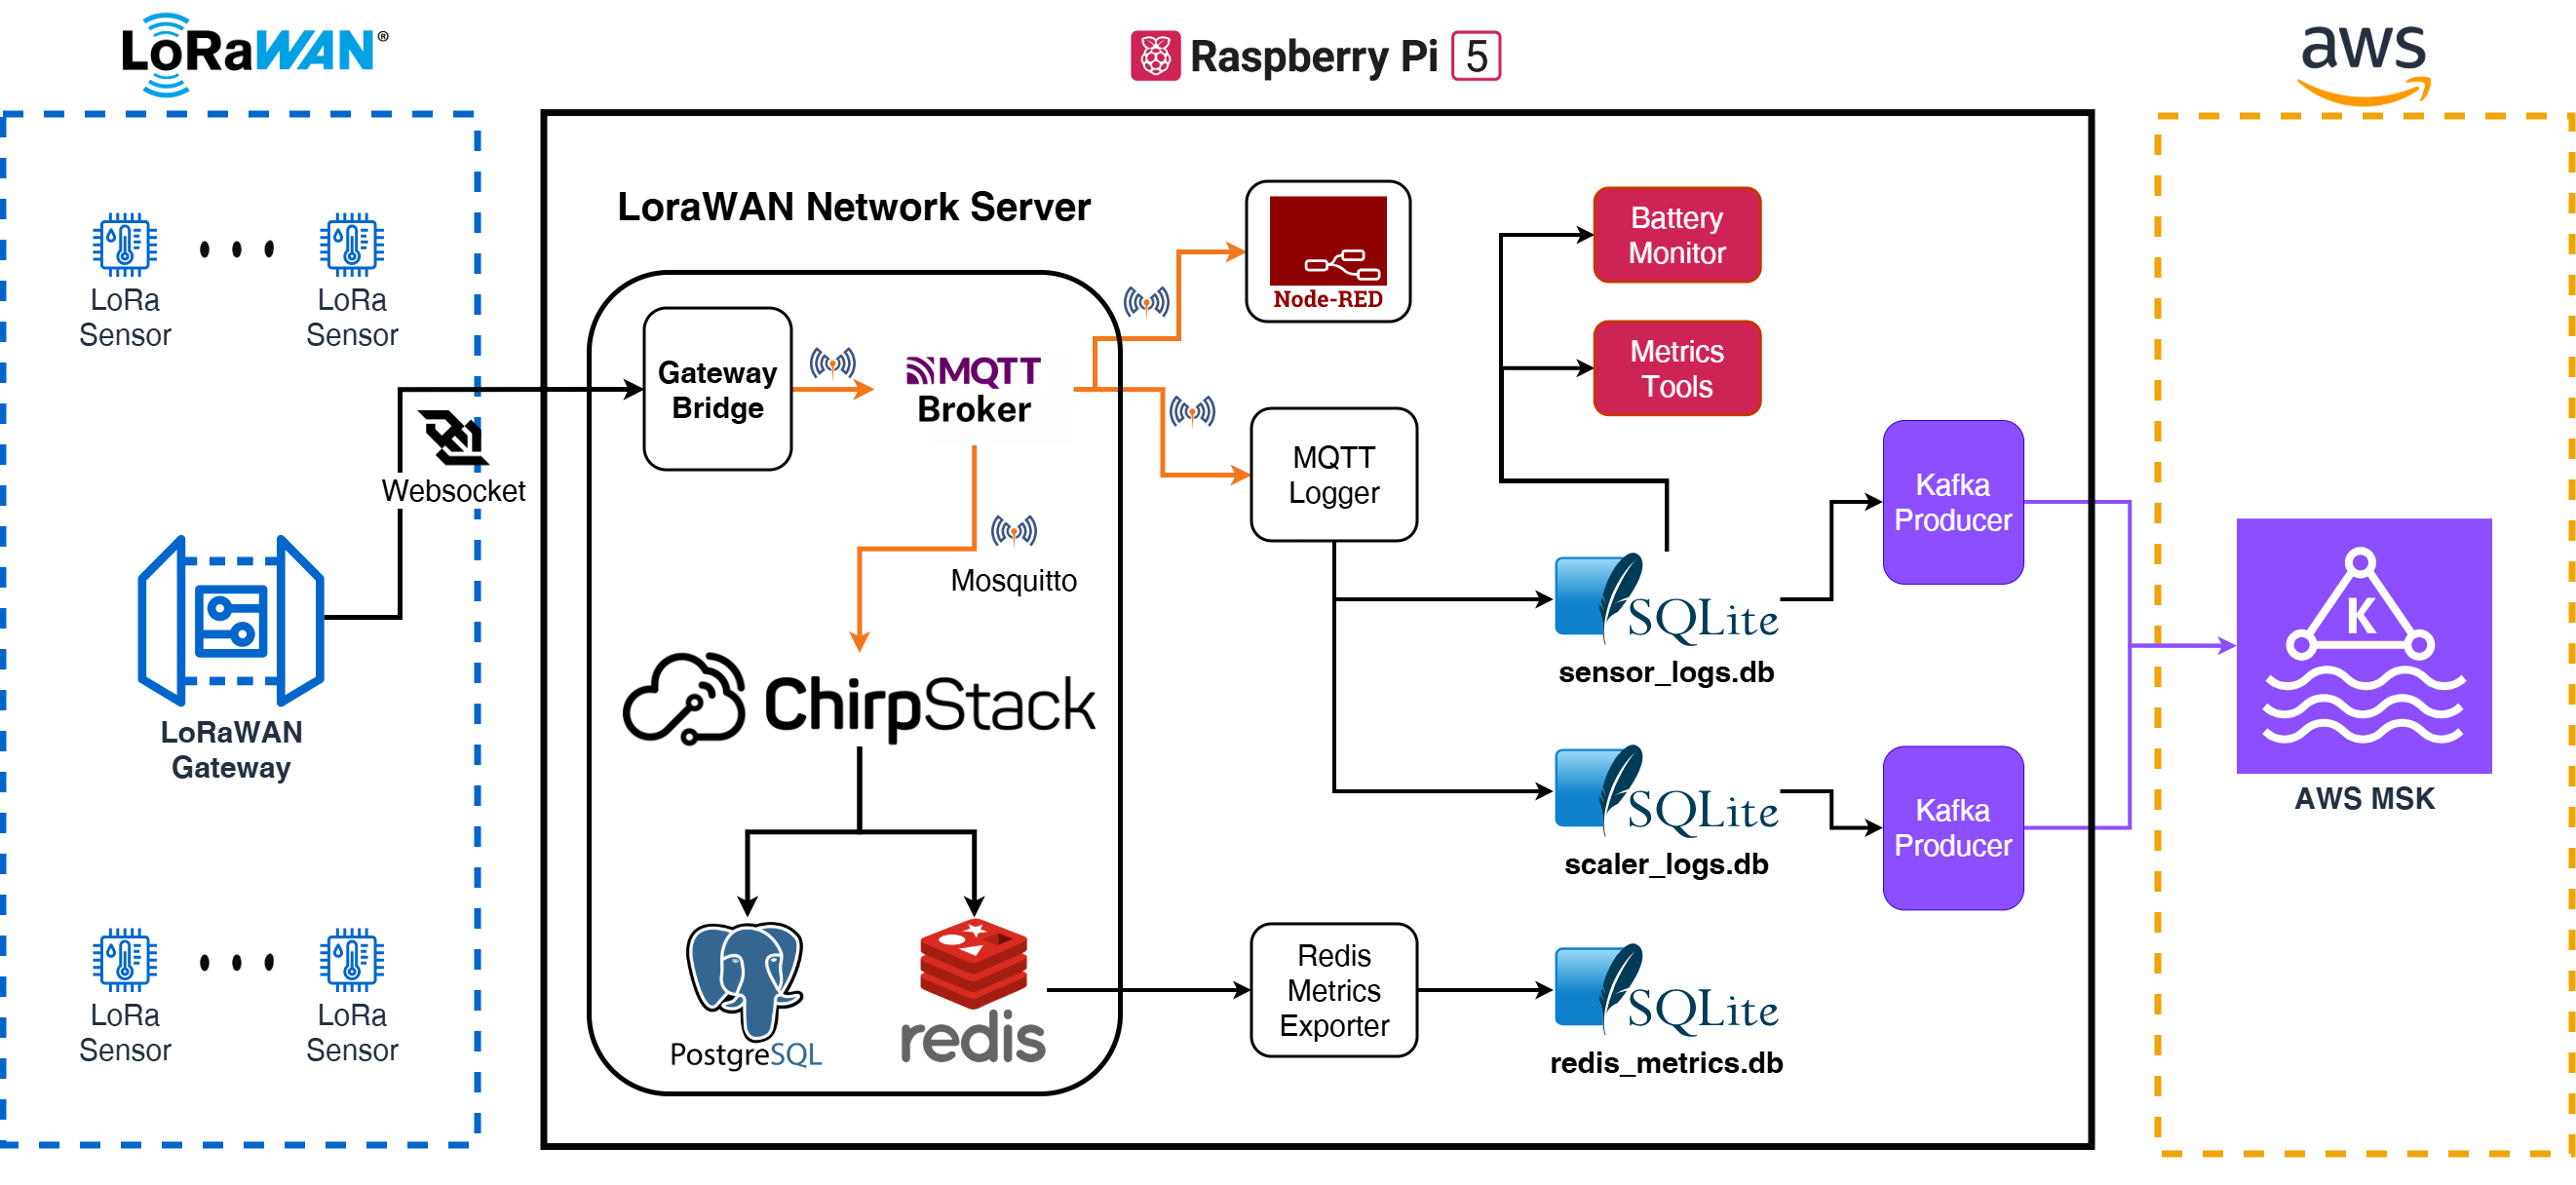
\includegraphics[width=1\linewidth]{figures/edge.png}
    \caption{Edge architecture for field data acquisition.}
    \label{fig:edge}
\end{figure}

The factory-side acquisition layer was implemented as an edge-centered intake stack that received field data inside the plant, preserved them locally, and then forwarded them to the cloud event pipeline. Because the plant did not provide a uniform network-native source environment or stable plant-wide connectivity across distributed process areas, the architecture was organized around a local edge boundary rather than direct source-to-cloud transmission.

LoRaWAN was selected as the field communication network because it allowed distributed source collection across the plant without extensive wiring and supported locally controlled operation under constrained factory conditions. Accordingly, the plant-side network was organized around LoRa uplinks converging on a local gateway and edge node.

As shown in Figure~\ref{fig:edge}, field events were transmitted through LoRa to the gateway, handled by ChirpStack Gateway Bridge and ChirpStack Server, relayed through an MQTT broker, and then accepted by edge-side services. On the edge node, MQTT logger and source-specific collectors wrote accepted records into local SQLite stores. This made the acquisition path explicit---field transmission, gateway reception, LoRaWAN handling, MQTT relay, edge logging, and upper-layer forwarding were treated as separate steps---and allowed the edge node to function as the first stable intake and persistence boundary of the system.

A central function of the edge stack was local persistence. Sensor uplinks accepted through MQTT were written to SQLite before cloud delivery was assumed, and additional edge-side components preserved operational traces needed to inspect collection quality and local failure modes. As a result, accepted field events first became durable inside the factory rather than remaining only as transient in-flight messages.

The edge stack also accommodated heterogeneous source conditions. A representative example was the production electronic scale, which did not provide native network communication. Its printer port was connected to the Raspberry Pi through an RS232 serial link, and a dedicated daemon collector parsed the incoming weighing values, stored them locally, and transmitted them through a LoRa device attached to the Raspberry Pi so that they could enter the same acquisition path as other field events. In practical terms, this flow can be summarized as \emph{Scale $\rightarrow$ RS232 $\rightarrow$ RPi $\rightarrow$ LoRa}. This showed that the edge architecture could absorb not only standard wireless sensor uplinks but also non-networked legacy equipment within the same factory-side event flow.

Once accepted and retained at the edge, the records were forwarded by producer services to the cloud broker layer. In the broader architecture, this upstream path was organized around Kafka-based streaming, including AWS MSK on the cloud side, so that raw events from each factory could be published into a shared event pipeline for subsequent parsing, normalization, and persistence. The next subsection explains that cloud-side processing path.

%%%%%%%%%%%%%%%%%%%%%%%%%%%%%%%%%%%%%%%%%%
\subsection{Cloud Processing Architecture}

\begin{figure}
    \centering
    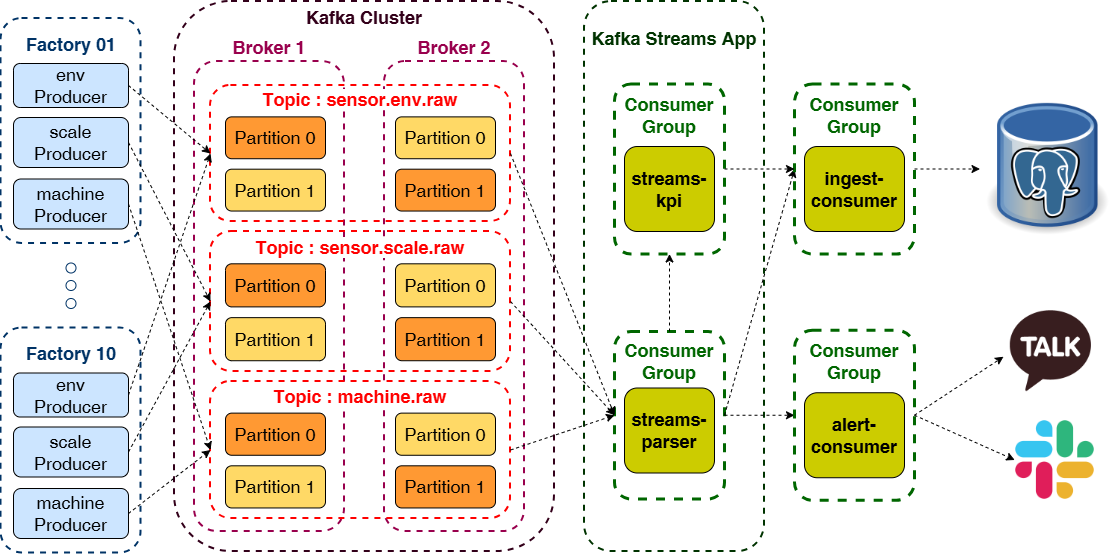
\includegraphics[width=1\linewidth]{figures/kafka.png}
    \caption{Cloud-side processing architecture.}
    \label{fig:kafka}
\end{figure}

On top of the field acquisition layer, the system implemented a cloud-side processing architecture designed to interpret, derive, persist, and serve the collected data. The end-to-end flow connected edge producers, a message broker, parser streams, KPI streams, ingest consumers, a database layer, and downstream dashboard and alert services. Rather than concentrating all responsibilities in a single application, this architecture separated message intake, semantic normalization, derived computation, persistence, and service consumption into distinct functional stages.

A central design objective of this architecture was functional decoupling. Producer-side acquisition was not allowed to depend directly on parser execution, KPI computation speed, or database ingestion performance, because failures in downstream stages should not immediately halt the upstream intake path. For this reason, a brokered event flow was adopted to decouple acquisition from later processing. The architectural significance of the message broker was therefore not simply that Kafka was used, but that the acquisition path and the processing path were separated so that failure propagation could be reduced and downstream evolution could proceed more independently.

The parser stage consumed raw topics and performed decoding, source mapping, metric unification, timestamp handling, deduplication, and canonical event generation. Raw inputs such as \texttt{sensor.env.raw}, \texttt{sensor.scale.raw}, and \texttt{machine.raw} were transformed into a unified canonical stream. The function of the parser was not to forward device-specific payloads downstream, but to convert heterogeneous source messages into a common semantic form that later stages could consume without direct knowledge of device-specific structure.

After normalization, a dedicated KPI stream consumed canonical events and generated derived indicators such as production quantity and yield. KPI computation was intentionally separated from the parser stage and from query-time dashboard logic so that raw normalization and business-level derivation remained distinct responsibilities. This separation reduced semantic overloading in the parser, isolated derived computation from storage concerns, and preserved the possibility of replay under changed KPI rules.

The outputs of the parser and KPI streams were then delivered to the database through ingest consumers. These consumers were designed primarily as an append-only persistence path rather than as another transformation layer. In other words, semantic interpretation and derived computation remained in the stream layer, while the persistence layer focused on durable storage of already-governed events. This design preserved separation between processing logic and storage logic and supported later reprocessing and reuse.

The cloud architecture also maintained clear deployment boundaries. Shared event contracts were placed in a common module, while producers, parser streams, KPI streams, and ingest services were separated into unidirectional dependencies. Consumer-side components were kept lightweight and stateless where possible, while stateful processing responsibility remained with the broker and stream-processing layers. Taken together, the cloud stack was not merely a path for relaying raw events, but a governed, replay-aware, and service-ready processing architecture built on top of the continuity secured at the field edge.




\begin{table}[H]
\caption{Cloud-side components and responsibilities.\label{tab:cloud_components_responsibilities}}
\begin{tabularx}{\textwidth}{
>{\raggedright\arraybackslash}X
>{\raggedright\arraybackslash}X
>{\raggedright\arraybackslash}X
>{\raggedright\arraybackslash}X}
\toprule
\textbf{Component} & \textbf{Input} & \textbf{Output} & \textbf{Primary responsibility} \\
\midrule

Producer
& Edge-side records/messages
& Raw topics
& Forward field data to the cloud event flow \\

Parser stream
& Raw topics
& Canonical events
& Decode, normalize, map sources, and standardize events \\

KPI stream
& Canonical events
& KPI events
& Derive production- and process-level indicators \\

Ingest consumer
& Canonical events, KPI events
& Database records
& Persist processed events without adding business logic \\

Database
& Ingested records
& Queryable tables/views
& Provide persistent storage for dashboards, alerts, and analysis \\

Dashboard/alert layer
& Stored and derived data
& Operational interfaces
& Present status, alarms, and management views \\

\bottomrule
\end{tabularx}
\end{table}


%%%%%%%%%%%%%%%%%%%%%%%%%%%%%%%%%%%%%%%%%%
\subsection{Data Model}

The data model was designed to provide stable semantics and replayable structure across heterogeneous sources. In a field environment where devices, payload formats, and process contexts differ substantially, exposing raw messages directly to downstream systems would have dispersed interpretation responsibility across the pipeline. For this reason, the implementation introduced a canonical event contract that internalized governance into the data path itself. The data model should therefore be understood not merely as a schema design choice, but as a structural mechanism for semantic control.

Each source was represented through a canonical identity organized around \texttt{source\_id}, including attributes such as \texttt{tenant\_id}, \texttt{line\_id}, \texttt{process}, \texttt{device\_type}, and \texttt{metric}. This identifier functioned as a semantic anchor rather than as a simple storage key. It allowed downstream components to operate on controlled source meaning without depending on raw device names or payload-specific fields, while a metadata layer preserved the source context in interpretable form.

Time semantics were also explicitly stabilized. In environments where sensor time, gateway time, network-server time, and receipt time may coexist, aggregation, deduplication, and persistence can become ambiguous if no common temporal reference is fixed. In this implementation, \texttt{edge\_ingest\_time} was used as the common pipeline reference time, while \texttt{event\_time}, \texttt{edge\_ingest\_time}, and \texttt{db\_ingest\_time} were stored as distinct time axes with different roles. This separation prevented confusion between raw occurrence time, pipeline reference time, and durable persistence time, and supported consistent timestamp interpretation across the entire processing path.

Canonical events were generated not through simple field copying, but through normalization rules that included metric unification, value-type alignment, deduplication, and explicit missing-value handling. Deduplication was performed in the parser stream rather than in producers or at the database layer, using ordering and key-based logic appropriate to the message stream. At the same time, the implementation distinguished true zero values from missing observations and minimized unnecessary \texttt{null} propagation in canonical records. These rules were important not as isolated data-cleaning tricks, but as operational rules for preserving stable downstream meaning.

Storage was organized as a layered structure rather than as a single undifferentiated table space. Canonicalized records were written into raw-domain tables such as \texttt{raw.sensor\_env}, \texttt{raw.sensor\_scale}, and \texttt{raw.machine}; source interpretation metadata were stored in \texttt{meta.source}; and derived KPI events were stored in \texttt{derived.kpi}. This organization separated raw-like canonical persistence from business-level derivation and thus preserved the distinction between governed operational records and derived management logic.

The resulting model supported replayability and future change. Because the structure preserved a raw-to-canonical-to-derived chain, parser rules or KPI logic could be revised without collapsing the semantic basis of historical records. The combination of a common event contract, append-only ingest, and layered storage was therefore not a purely implementation-specific choice, but a structural condition for reprocessability and evolvability. At the same time, it provided the persistence basis on which dashboards, alerts, and other operational interfaces could be built.

%%%%%%%%%%%%%%%%%%%%%%%%%%%%%%%%%%%%%%%%%%
\subsection{Operations and Control}

The implementation did not stop at data capture and storage. It was also connected to an operational layer through which plant operators and managers could observe state, receive alerts, and intervene when necessary. In this sense, the system was designed not as a hidden back-end pipeline, but as a data foundation that could be translated into operational visibility and action.

Dashboards provided real-time and cumulative views of temperature, humidity, weight, device status, battery condition, packet reception status, and derived KPIs. These views were not designed as raw-signal viewers alone, but as visual interfaces that reorganized operational data into line charts, status summaries, alert histories, and key figures suitable for day-to-day plant awareness. As a result, operators could inspect process conditions, environmental changes, sensor stability, and production-related indicators without relying solely on manual records.

The system also included an alert path for operational intervention. Threshold violations, prolonged silence from data sources, battery-related conditions, and other abnormal states were delivered as asynchronous alerts so that operators could respond promptly. Alert history was preserved alongside the dashboard layer, allowing visual monitoring and intervention support to remain linked rather than isolated. In this design, alerting was not treated as an accessory to monitoring, but as the path through which recognized states became actionable events.

Beyond immediate visibility, the processed and stored data also supported KPI tracking, reporting, and management-level review. Because raw-domain and derived layers were both preserved, the implementation supported not only real-time state checking, but also historical comparison, accumulation-based reporting, and line- or period-level operational review. The dashboard layer therefore served both operator-level situational awareness and manager-level visibility grounded in the same governed data basis.

The implementation further extended to machine-side control capability. The system was built to support actual power control of machinery in the field, meaning that it was capable not only of observing states and issuing alerts, but also of participating in operational intervention. This does not imply that the study centered on control automation itself; rather, it demonstrates that the operational data foundation had already reached the point where downstream device action could be connected to the same semantic and operational chain.

Overall, the operational layer linked dashboards, alerts, KPIs, and machine-side intervention on top of a single governed data foundation. This makes the implemented system more than a data collection pipeline: it functions as an operational interface through which perception, interpretation, response, and future application expansion can be organized on a common basis. The next section evaluates how this implementation satisfies the requirements and invariants defined in Section~4.





%%%%%%%%%%%%%%%%%%%%%%%%%%%%%%%%%%%%%%%%%%
%%%%%%%%%%%%%%%%%%%%%%%%%%%%%%%%%%%%%%%%%%
\section{Evaluation of the Framework}





This section evaluates whether the proposed framework functioned as an operational data foundation in a real manufacturing setting. The evaluation does not focus on conventional system benchmarking or algorithmic accuracy. Instead, it examines how the six framework requirements---continuity, governance, diagnosability, operability, reprocessability, and evolvability---became visible in the implemented system and in its operational history. Accordingly, Section~6.1 summarizes requirement-wise evidence, and Section~6.2 presents a representative field case in which continuity and diagnosability were most directly tested through the diagnosis and improvement of LoRa reception instability.

%%%%%%%%%%%%%%%%%%%%%%%%%%%%%%%%%%%%%%%%%%
\subsection{Framework Compliance}

This subsection assesses the framework in terms of the six core requirements defined in Section~4. Rather than reducing each requirement to a single metric, the assessment draws on multiple forms of evidence, including source identity structure, time semantics, layered persistence, segment-wise observability, intervention history, and historical data retention. Table~\ref{tab:requirement_evidence_significance} summarizes the main evidence for each requirement and its significance, while the discussion below interprets these observations in operational terms.



\begin{table}[H]
\caption{Requirement-wise evidence and significance.\label{tab:requirement_evidence_significance}}
\begin{tabularx}{\textwidth}{
>{\raggedright\arraybackslash}X
>{\raggedright\arraybackslash}X
>{\raggedright\arraybackslash}X}
\toprule
\textbf{Requirement} & \textbf{Key evidence} & \textbf{Significance} \\
\midrule

Continuity
& local capture, recovery path, reception improvement
& recoverable continuity \\

Governance
& canonical schema, source identity, time semantics
& controlled and traceable meaning \\

Diagnosability
& segment-wise metrics, gateway-to-DB discrepancy visibility
& localizable and actionable failures \\

Operability
& deployable modular stack, monitoring/control interfaces
& manageable field operation \\

Reprocessability
& preserved raw data, layered storage
& recomputation and correction \\

Evolvability
& extensible source model, modular interfaces
& incremental expansion \\

\bottomrule
\end{tabularx}
\end{table}




\textbf{Continuity} was evaluated not as the perfect arrival of every event, but as the extent to which the event flow remained traceable and recoverable under unstable field conditions. In the implemented system, gateway reception, edge-side logging, downstream ingest, and database persistence could be observed as separate stages, allowing continuity to be interpreted through persisted-to-expected ratios, extended no-data intervals, and before--after improvement patterns. Under an expected daily volume of roughly 48{,}000 events, early persistence remained near 15{,}800 events, and some source groups exhibited repeated no-data gaps of 2--5 hours. After communication-related adjustments, persisted events recovered to approximately 45{,}600 per day, while extended gaps decreased from about 18 cases per day to fewer than two. These observations indicate that continuity in this system was not merely a matter of raw transmission success, but of maintaining a recoverable operational record despite intermediate instability.

\textbf{Governance} was reflected in whether heterogeneous field messages could be preserved and interpreted under a stable semantic discipline rather than being stored as loosely structured payloads. In the implemented system, source identity was organized around \texttt{source\_id}, while the parser stage fixed metric normalization, timestamp normalization, deduplication, and missing-value handling before downstream use. The distinction among \texttt{event\_time}, \texttt{edge\_ingest\_time}, and \texttt{db\_ingest\_time} prevented ambiguity between occurrence, pipeline reference, and persistence time. In addition, the separation of raw-like persistence from derived KPI layers preserved a stable semantic boundary between operational records and business-level interpretation. Taken together, these structures show that governance was realized as controlled meaning across collection, normalization, and storage.

\textbf{Diagnosability} was evaluated in terms of whether data loss or delay remained a black-box symptom or could be localized to specific lifecycle segments. Because gateway-visible counts, local logs, parser/consumer stages, and database persistence counts could be compared, the same symptom of ``too little data'' could be interpreted as distinct failure modes. In some intervals, gateway-visible counts were already well below expectations, directing attention to upstream collection and communication; in other situations, the discrepancy widened between gateway-visible counts and persisted records, indicating the need to inspect downstream processing or storage. This segment-wise visibility was especially important in the LoRa case discussed in Section~6.2, where the main source of degradation could be narrowed to the communication-configuration layer rather than being misread as a parser or database issue.

\textbf{Operability} was reflected not merely in technical feasibility, but in whether the system could be deployed, inspected, tuned, and maintained under limited staffing and maintenance capacity. The implementation separated field-side acquisition, gateway and network services, edge persistence, cloud processing, database storage, and dashboard/alert interfaces by function, reducing unnecessary entanglement among acquisition, normalization, storage, derivation, and presentation. In actual operation, interventions such as rejoin handling, configuration adjustment, logging verification, interval tuning, and packet comparison could be performed at the relevant layer without redesigning the system as a whole. This indicates that the structure remained operationally manageable beyond a laboratory prototype and could be sustained under realistic factory conditions.

\textbf{Reprocessability} was assessed in terms of whether collected data remained available for future reinterpretation, recalculation, correction, and recovery rather than being consumed only by the current dashboard or rule logic. The implemented system avoided transformed-only persistence by separating raw-like event storage, source metadata, and derived KPI layers. As a result, historical records remained available for parser rule revision, KPI redefinition, historical audit, and retrospective reconstruction. The accumulated historical storage reached roughly 0.84--1.57 million rows, indicating that the system functioned not only as a short-term monitoring pipeline but also as a retained operational record base capable of supporting later reprocessing needs.

\textbf{Evolvability} was reflected in whether the structure could accept additional sources, process-specific measurements, monitoring tools, KPI logic, and downstream services without breaking its prevailing governance discipline. Because the system was organized around a common event contract, source identity discipline, parser-stage normalization, and modular responsibility separation, new sources could be incorporated primarily through onboarding rules and parser extensions rather than through full pipeline redesign. During the project, additional source classes, monitoring tools, derived KPI layers, and dashboard/alert functions were progressively introduced while the overall structure remained intact. This indicates that the framework supported staged expansion rather than one-time integration only.

Taken together, the evidence above shows that the proposed framework was realized not only as a conceptual structure but as an operational one. Among the six requirements, continuity and diagnosability were tested most directly through actual field instability, and their operational relevance becomes especially clear in the representative case discussed next.

%%%%%%%%%%%%%%%%%%%%%%%%%%%%%%%%%%%%%%%%%%
\subsection{Operational Case: LoRa Reliability Improvement}

A field data foundation does not remain stable simply because it has once been installed. In practice, reception quality, device condition, battery state, wireless configuration, and operational usage patterns continue to change over time. For this reason, the value of the proposed framework lies not in whether it delivered perfect performance from the outset, but in whether it enabled emerging failures to be detected, localized, and corrected in an operationally meaningful way. This subsection presents a representative case in which severe reception degradation in periodic uplink collection was diagnosed and improved through the framework’s continuity and diagnosability logic.

During the early operation period, the plant-wide event flow failed to maintain the expected level of periodic collection, and reception rates in some source groups dropped to roughly 33\%. Under an expected daily volume of around 48{,}000 events, persisted events remained near 15{,}800, and repeated no-data intervals of 2--5 hours appeared in some groups. This was not merely a matter of lower communication quality. It directly weakened line-level visibility, reduced confidence in dashboard and alert outputs, and undermined the continuity of the operational record.

Because the implemented system did not rely solely on final database status, this degradation could be interpreted as a segment-wise discrepancy rather than as a vague end-to-end symptom. Gateway-visible counts, local edge logs, parser/consumer stages, and database persistence counts could be examined together. In one representative 24-hour window, gateway-visible events were already only about 16{,}400, far below expectation, whereas the persistence ratio from gateway-visible events to database records remained around 97--99\%. This pattern suggested that the main problem lay upstream of parsing and storage, making it more reasonable to investigate the collection and communication segment first.

Through this segment-wise diagnosis, the dominant cause was gradually localized not to parser failure or database loss, but to reception instability associated with the communication-configuration layer. In particular, the combination of confirmed mode, dependence on downlink acknowledgements, and limited channel availability was interpreted as a major source of degradation. In LoRa environments, confirmed uplinks require network-side downlink ACKs. When many field devices transmit at short intervals, downlink resources can become saturated, ACK delays or omissions accumulate, and retransmissions increase contention. Under such conditions, the visible symptom is uplink instability, but the underlying bottleneck is often downlink saturation. For example, if 60 field devices transmit every 5 minutes, the expected uplink load is about 720 messages per hour; even a 25\% ACK miss rate can raise retransmission-induced traffic substantially and worsen congestion.

Once the likely bottleneck had been localized to the communication layer, the response proceeded through targeted intervention rather than unguided trial and error. The main adjustments included relaxation of confirmed-mode dependence, expansion of active channels, device rejoin, transmission-parameter tuning, and refinement of monitoring intervals. Each change corresponded to a specific bottleneck hypothesis, allowing recovery effects to be interpreted in relation to the observed loss pattern. The concrete configuration changes and their intended effects are summarized in Table~\ref{tab:segmentwise_event_counts}.



\begin{table}[H]
\caption{Event counts across pipeline segments during reception degradation.\label{tab:segmentwise_event_counts}}
\begin{tabularx}{\textwidth}{
>{\raggedright\arraybackslash}X
>{\raggedleft\arraybackslash}X
>{\raggedleft\arraybackslash}X
>{\raggedleft\arraybackslash}X}
\toprule
\textbf{Stage / Metric} & \textbf{Expected} & \textbf{Observed} & \textbf{Ratio (\%)} \\
\midrule

Scheduled transmissions
& 48{,}000
& --
& -- \\

Gateway-visible events
& 48{,}000
& 16{,}400
& 34.2 \\

Edge/local logged events
& 16{,}400
& 16{,}120
& 98.3 \\

Ingested events
& 16{,}120
& 15{,}980
& 99.1 \\

DB-persisted events
& 15{,}980
& 15{,}870
& 99.3 \\

\bottomrule
\end{tabularx}
\end{table}




After these adjustments, collection stability improved markedly. Packet reception increased from approximately 33\% to 95\%, daily persisted events rose from about 15{,}800 to 45{,}600, extended no-data intervals decreased from about 18 cases per day to fewer than two, and average gap duration dropped from roughly 145 minutes to 18 minutes. Time-series plots also showed that dense missing segments visible before adjustment were substantially reduced afterward, while observation regularity and line-to-line consistency improved (Figure~\ref{fig:reception}; Table~\ref{tab:reception_improvement_outcome}).

The significance of this case extends beyond successful LoRa tuning. It demonstrates that continuity degradation could be made observable, that the dominant cause could be narrowed to a specific lifecycle segment, and that the effects of intervention could be re-evaluated within the same operational structure. Continuity was revealed through degradation and recovery, diagnosability through segment-wise discrepancy visibility, and operability through configuration-based field intervention. Governance also mattered, because packet flow could be compared by source group and time window rather than only through aggregate counts. In this sense, the case shows that the proposed framework functioned not merely as a storage path, but as a problem-solving foundation that enabled unexpected field failures to be translated into operationally actionable improvement.



\begin{figure}[H]
    \centering
    \subfloat[\centering\label{fig:reception_before}]{
        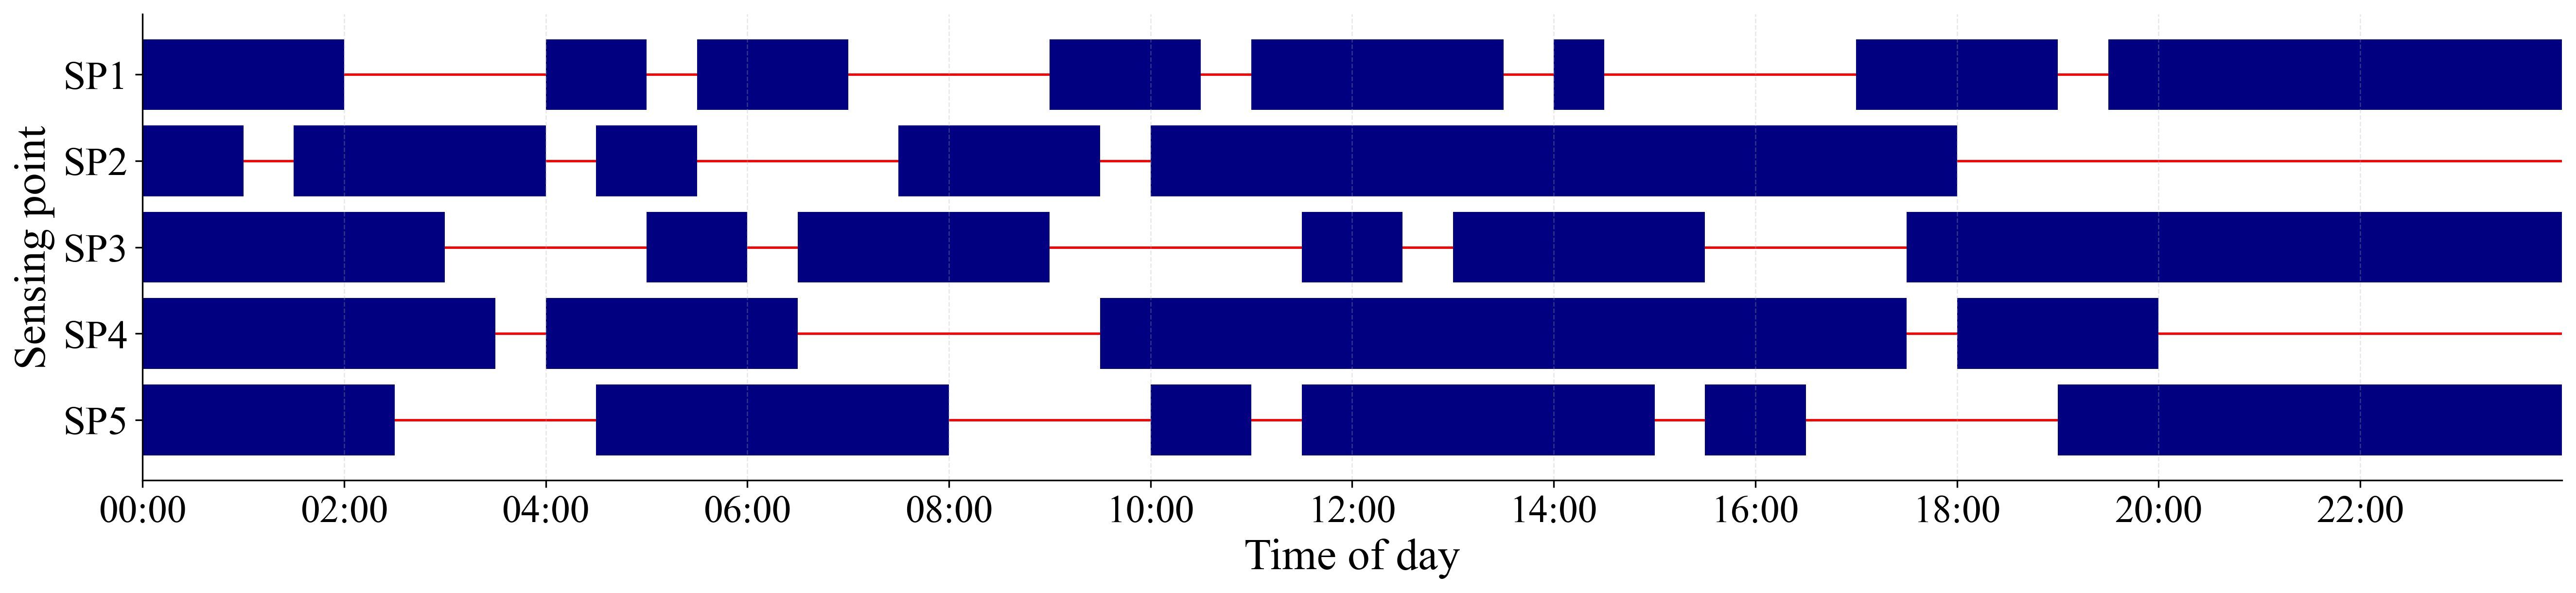
\includegraphics[width=\linewidth]{figures/figure6_2_before_adjustment.png}
    }\\[0.7em]
    \subfloat[\centering\label{fig:reception_after}]{
        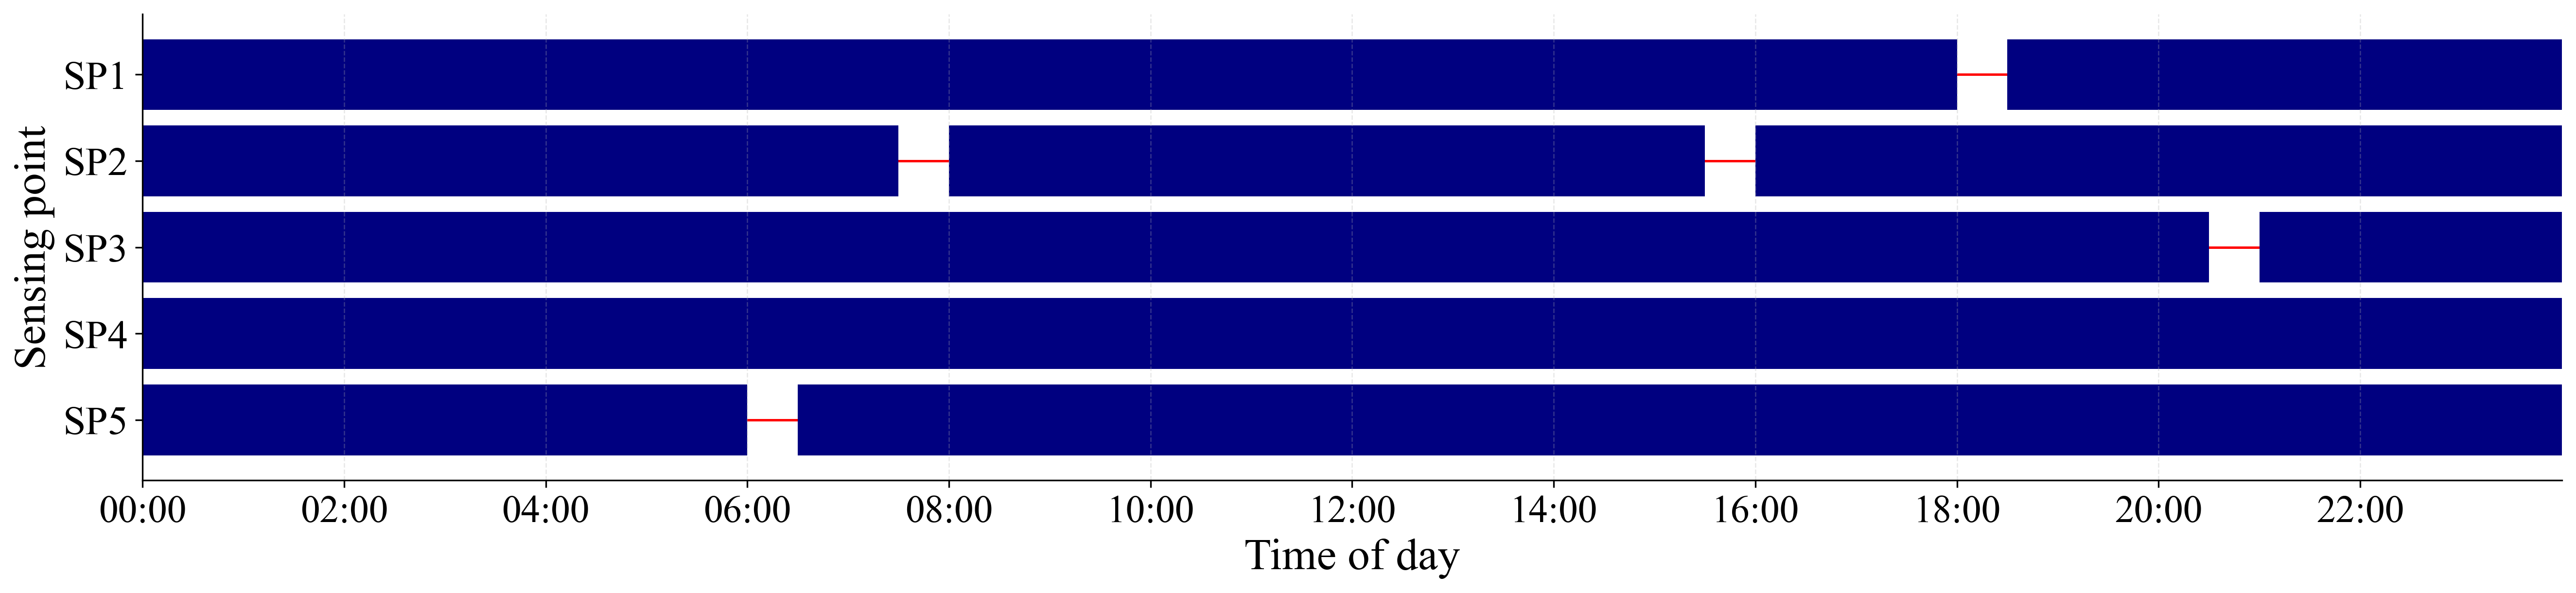
\includegraphics[width=\linewidth]{figures/figure6_2_after_adjustment.png}
    }
    \caption{Reception stability across sensing points over time. (\textbf{a}) Before adjustment. (\textbf{b}) After adjustment.}
    \label{fig:reception_stability}
\end{figure}



\begin{table}[H]
\caption{Outcome of reception reliability improvement.\label{tab:reception_improvement_outcome}}
\begin{tabularx}{\textwidth}{
>{\raggedright\arraybackslash}X
>{\raggedleft\arraybackslash}X
>{\raggedleft\arraybackslash}X
>{\raggedleft\arraybackslash}X}
\toprule
\textbf{Metric} & \textbf{Before} & \textbf{After} & \textbf{Change} \\
\midrule

Reception rate (\%)
& 33
& 95
& +62 pp \\

Persisted events/day
& 15{,}870
& 45{,}600
& +187\% \\

Average gap duration (min)
& 145
& 18
& --87.6\% \\

Long-gap events/day
& 18
& 2
& --88.9\% \\

Gateway-to-DB consistency (\%)
& 96.8
& 99.4
& +2.6 pp \\

\bottomrule
\end{tabularx}
\end{table}




%%%%%%%%%%%%%%%%%%%%%%%%%%%%%%%%%%%%%%%%%%
%%%%%%%%%%%%%%%%%%%%%%%%%%%%%%%%%%%%%%%%%%
\section{Conclusion}

This study argued that the practical bottleneck of smart manufacturing in constrained SME factories lies not only in downstream analytics or intelligent applications, but more fundamentally in the absence of an operationally viable data foundation. In such environments, legacy equipment, fragmented systems, unstable field conditions, limited staffing, and cost sensitivity weaken the assumptions on which idealized smart manufacturing architectures are often built. The central question, therefore, is not simply how to use more data, but how to design and sustain a data foundation that remains operationally viable under real deployment conditions.

To address this problem, this study proposed the \emph{Operational Data Foundation Framework} for constrained SME factories. The framework formalized six core requirements---continuity, governance, diagnosability, operability, reprocessability, and evolvability---and connected them to corresponding design principles and operational invariants. In this way, the study contributed not merely a particular architecture, but a structured framework that links problem analysis, design logic, and assessment criteria for operational data foundations in smart manufacturing systems.

The framework was then instantiated in a real SME food-manufacturing deployment and evaluated from the perspective of operational viability rather than benchmark performance alone. Through requirement-based evidence and a representative field case, the study showed that the framework remained operationally meaningful in practice. In particular, the diagnosis and improvement of LoRa reception instability demonstrated that continuity and diagnosability were not abstract design goals, but directly relevant to the detection, interpretation, and correction of real operational problems.

More broadly, this study did not seek to add another downstream smart manufacturing application. Instead, it formalized the operational data foundation on which such applications depend. In this sense, the proposed framework provides a reference design logic for building data systems that can support real-time monitoring, traceability, analytics, alerting, and future extensions toward more adaptive and integrated manufacturing systems. Its contribution is therefore both practical and conceptual: it offers a field-grounded way to think about data-system design under constrained deployment conditions.

This study has several limitations. The framework was examined through a single SME food-manufacturing deployment, and its broader generalizability across multiple factories and more diverse industrial settings remains to be tested. In addition, although the implementation supported operational visibility, alerting, and machine-side intervention, the study did not directly evaluate large-scale multi-site deployment, fully automated replay workflows, or closed-loop control integration. Future work may therefore extend the framework through multi-factory replication, richer interoperability settings, automated regeneration and replay pipelines, and tighter integration with analytics, digital twins, and CPPS-oriented control.




%%%%%%%%%%%%%%%%%%%%%%%%%%%%%%%%%%%%%%%%%%
\vspace{6pt} 


%%%%%%%%%%%%%%%%%%%%%%%%%%%%%%%%%%%%%%%%%%
\authorcontributions{For research articles with several authors, a short paragraph specifying their individual contributions must be provided. The following statements should be used ``Conceptualization, X.X. and Y.Y.; methodology, X.X.; software, X.X.; validation, X.X., Y.Y. and Z.Z.; formal analysis, X.X.; investigation, X.X.; resources, X.X.; data curation, X.X.; writing---original draft preparation, X.X.; writing---review and editing, X.X.; visualization, X.X.; supervision, X.X.; project administration, X.X.; funding acquisition, Y.Y. All authors have read and agreed to the published version of the manuscript.'', please turn to the  \href{http://img.mdpi.org/data/contributor-role-instruction.pdf}{CRediT taxonomy} for the term explanation. Authorship must be limited to those who have contributed substantially to the work~reported.}

\funding{Please add: ``This research received no external funding'' or ``This research was funded by NAME OF FUNDER grant number XXX.'' and  and ``The APC was funded by XXX''. Check carefully that the details given are accurate and use the standard spelling of funding agency names at \url{https://search.crossref.org/funding}, any errors may affect your future funding.}

\dataavailability{We encourage all authors of articles published in MDPI journals to share their research data. In this section, please provide details regarding where data supporting reported results can be found, including links to publicly archived datasets analyzed or generated during the study. Where no new data were created, or where data is unavailable due to privacy or ethical restrictions, a statement is still required. Suggested Data Availability Statements are available in section ``MDPI Research Data Policies'' at \url{https://www.mdpi.com/ethics}.} 

\acknowledgments{In this section you can acknowledge any support given which is not covered by the author contribution or funding sections. This may include administrative and technical support, or donations in kind (e.g., materials used for experiments). Where GenAI has been used for purposes such as generating text, data, or graphics, or for study design, data collection, analysis, or interpretation of data, please add “During the preparation of this manuscript/study, the author(s) used [tool name, version information] for the purposes of [description of use]. The authors have reviewed and edited the output and take full responsibility for the content of this publication.”}

\conflictsofinterest{The authors declare no conflicts of interest.} 


%%%%%%%%%%%%%%%%%%%%%%%%%%%%%%%%%%%%%%%%%%
%\isPreprints{}{% This command is only used for ``preprints''.
\begin{adjustwidth}{-\extralength}{0cm}
%} % If the paper is ``preprints'', please uncomment this parenthesis.
%\printendnotes[custom] % Un-comment to print a list of endnotes

\reftitle{References}

% Please provide either the correct journal abbreviation (e.g. according to the “List of Title Word Abbreviations” http://www.issn.org/services/online-services/access-to-the-ltwa/) or the full name of the journal.
% Citations and References in Supplementary files are permitted provided that they also appear in the reference list here. 


\bibliography{references}



% If authors have biography, please use the format below
%\section*{Short Biography of Authors}
%\bio
%{\raisebox{-0.35cm}{\includegraphics[width=3.5cm,height=5.3cm,clip,keepaspectratio]{Definitions/author1.pdf}}}
%{\textbf{Firstname Lastname} Biography of first author}
%
%\bio
%{\raisebox{-0.35cm}{\includegraphics[width=3.5cm,height=5.3cm,clip,keepaspectratio]{Definitions/author2.jpg}}}
%{\textbf{Firstname Lastname} Biography of second author}


\PublishersNote{}
%\isPreprints{}{% This command is only used for ``preprints''.
\end{adjustwidth}
%} % If the paper is ``preprints'', please uncomment this parenthesis.
\end{document}

